% !TEX program = lualatex
% A standalone manuscript. Run lualatex twice, or latexmk -lualatex blueprint.tex.
\documentclass[10pt,a4paper]{article}
\usepackage[top=23mm,bottom=23mm,left=24mm,right=24mm,headheight=14pt,headsep=9mm]{geometry}
\usepackage{fontspec,amsmath,unicode-math}
\setmainfont{LibertinusSerif-Regular.otf}[BoldFont=LibertinusSerif-Semibold.otf,ItalicFont=LibertinusSerif-Italic.otf,BoldItalicFont=LibertinusSerif-BoldItalic.otf]
\setsansfont{LibertinusSans-Regular.otf}[BoldFont=LibertinusSans-Bold.otf,ItalicFont=LibertinusSans-Italic.otf]
\setmathfont{LibertinusMath-Regular.otf}
\directlua{luaotfload.add_fallback("blueprintcode", {"[STIXTwoMath-Regular.otf]:mode=base;", "[FreeSerif.ttf]:mode=base;"})}
\setmonofont{DejaVuSansMono.ttf}[BoldFont=DejaVuSansMono-Bold.ttf,ItalicFont=DejaVuSansMono-Oblique.ttf,RawFeature={fallback=blueprintcode},Scale=1.0]
\usepackage{microtype,xcolor,fvextra,fancyhdr,tabularx,booktabs,enumitem,etoolbox}
\usepackage[unicode,colorlinks=true,linkcolor=inkblue,citecolor=inkblue,urlcolor=inkblue,pdfdisplaydoctitle=true]{hyperref}
\usepackage{bookmark,tikz}
\usetikzlibrary{arrows.meta}
\tikzset{guidebox/.style={draw=inkblue,fill=inkblue!5,rounded corners=2pt,
             text width=3.02cm,align=center,inner sep=3.1pt,font=\footnotesize\sffamily},
         guidefinal/.style={guidebox,draw=inkblue,fill=inkblue!14,line width=1pt},
         guidearrow/.style={-{Stealth[length=1.7mm]},draw=inkblue!85,line width=.65pt}}
\definecolor{inkblue}{HTML}{20586A}
\definecolor{quiet}{HTML}{405052}
\definecolor{hairline}{HTML}{BCCACE}
\hypersetup{pdftitle={A conditional Diophantine definition of the integers in the rationals},
 pdfsubject={A numbered mathematical blueprint with Lean statements and proofs},pdfauthor={},
 pdfkeywords={Diophantine definability, rational numbers, elliptic curves, Prym varieties, Lean}}
\newcommand{\Q}{\mathbb Q}\newcommand{\Z}{\mathbb Z}\newcommand{\N}{\mathbb N}\newcommand{\C}{\mathbb C}
\DeclareMathOperator{\End}{End}
\newcommand{\sectitle}[1]{{\large\bfseries #1}\par}
\setlength{\parindent}{0pt}\setlength{\parskip}{3.2pt plus 0.7pt minus 0.3pt}
\setlength{\emergencystretch}{1.5em}
\setlength{\abovedisplayskip}{5pt plus 2pt}\setlength{\belowdisplayskip}{5pt plus 2pt}
\setcounter{tocdepth}{1}
\setlist[itemize]{nosep,leftmargin=1.22em}
\pagestyle{fancy}\fancyhf{}
\fancyhead[L]{\footnotesize\sffamily\color{quiet}\nouppercase{\leftmark}}
\fancyhead[R]{\footnotesize\sffamily\color{quiet}Diophantine definability}
\fancyfoot[C]{\small\thepage}
\renewcommand{\sectionmark}[1]{\markboth{\thesection.\quad#1}{}}
\renewcommand{\headrulewidth}{0.25pt}\renewcommand{\footrulewidth}{0pt}
\raggedbottom
\newcounter{claim}
\newsavebox{\entrybox}
\newcommand{\beginentry}[3]{%
  \par\addvspace{10pt plus 1pt minus 1pt}%
  \setbox\entrybox=\vbox\bgroup\hsize=\linewidth
  \refstepcounter{claim}\label{st:#1}%
  \pdfbookmark[2]{#2 \theclaim. #3}{outline.#1}%
  {\bfseries #2 \theclaim.\hspace{.43em}#3.}\par\nobreak}
\newcommand{\explain}[1]{\par\noindent\textit{#1.}\enspace}
\newcommand{\leanlink}[2]{\par\nobreak\noindent
  {\footnotesize\sffamily\href{#1}{#2}}\par\nobreak}
\DefineVerbatimEnvironment{leancode}{Verbatim}{fontsize=\fontsize{8.15}{10.4}\selectfont,breaklines=true,breakanywhere=true,breakautoindent=true,breakindent=1.3em,breaksymbolleft={},breaksymbolright={},samepage=false,xleftmargin=0.7em,baselinestretch=1,listparameters={\setlength{\topsep}{1.8pt}\setlength{\partopsep}{0pt}}}
\newcommand{\relations}[3]{\par\nobreak\noindent{\footnotesize\sffamily\color{quiet}%
  \ifstrempty{#2}{}{#1\enspace #2.\quad}%
  \ifstrempty{#3}{}{Used in\enspace #3.}}\par\egroup
  \ifdim\dimexpr\ht\entrybox+\dp\entrybox\relax>\textheight
    \unvbox\entrybox
  \else
    \box\entrybox
  \fi\par}
\newcommand{\primarysources}[1]{\par\noindent{\footnotesize\sffamily #1}\par\nobreak}
\newcommand{\paperlink}[2]{\href{#1}{\textit{#2}}}
\clubpenalty=8500\widowpenalty=8500
\begin{document}
\thispagestyle{empty}
\pdfbookmark[0]{A conditional Diophantine definition of the integers in the rationals}{title}
\vspace*{4mm}
{\fontsize{28}{32}\selectfont\bfseries A conditional Diophantine definition\\of the integers in the rationals\par}
\smallskip
{\large\color{quiet}A mathematical blueprint with Lean statements and proofs\par}
\vspace{6mm}
Let $t$ denote a rational number, and identify $\Z$ with its image in $\Q$. A subset of $\Q$ is Diophantine over $\Q$ if it is the projection of the rational zero set of a polynomial. For the integers, the polynomial in this definition can be required to have integer coefficients by clearing denominators.

\medskip
\textbf{Main theorem (conditional, Theorem~\hyperref[st:final]{\ref*{st:final}}).}
Assume the twelve propositions in the register on page~\pageref{register}. Then there exist $k\in\N$ and $P\in\Z[T,X_1,\ldots,X_k]$ such that for every $t\in\Q$,
\[
                   t\in\Z
       \quad\Longleftrightarrow\quad
                   \exists\,w\in\Q^k,\quad P(t,w)=0.
\]
The polynomial is chosen before $t$. The argument determines neither the number of witnesses nor the coefficients of a particular defining polynomial.

\medskip
Glazer and collaborators represent an integer by a multiple of a fixed elliptic point \cite{Glazer}. To recover the ordinary rational input from this representation, their argument uses a height inequality at six rational values. Here a genus-two pencil supplies an inequality of the required exponent with an unspecified uniform coefficient. One common field for the descent and one compatible choice of height over that field are essential. The \hyperref[roadmap]{Leitfaden} explains how the two uniform choices enter the proof.

\vfill
\begingroup
\renewcommand{\contentsname}{Contents}
\setlength{\parskip}{0pt}\tableofcontents
\endgroup
\clearpage
\phantomsection\label{roadmap}
\addcontentsline{toc}{section}{Leitfaden}
\markboth{Leitfaden}{}
\sectitle{Leitfaden}
The arithmetic argument asks for a point of infinite order on certain elliptic curves and one uniform estimate on the rational height. The geometry supplies this estimate. In the diagram each number opens the corresponding statement. An arrow may pass through intermediate lemmas.
\begin{center}
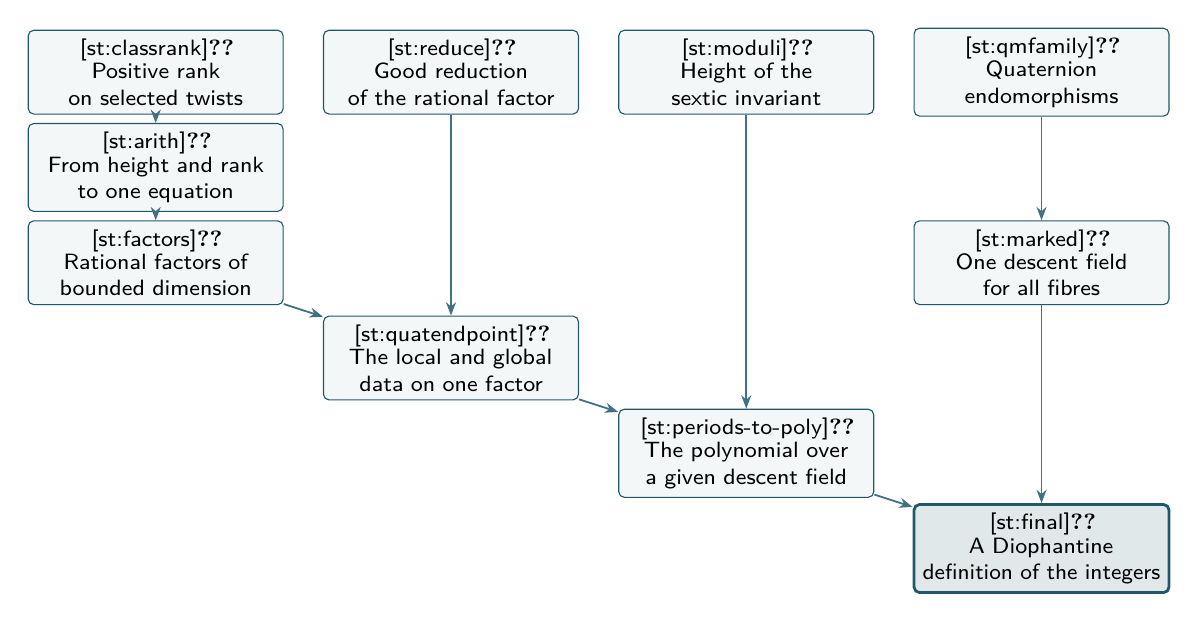
\begin{tikzpicture}[x=3.75cm,y=-1.21cm]
\node[guidebox] (classrank) at (0,0) {\hyperref[st:classrank]{\bfseries\ref*{st:classrank}}\\[-1pt]Positive rank\\on selected twists};
\node[guidebox] (reduce) at (1,0) {\hyperref[st:reduce]{\bfseries\ref*{st:reduce}}\\[-1pt]Good reduction\\of the rational factor};
\node[guidebox] (moduli) at (2,0) {\hyperref[st:moduli]{\bfseries\ref*{st:moduli}}\\[-1pt]Height of the\\sextic invariant};
\node[guidebox] (qmfamily) at (3,0) {\hyperref[st:qmfamily]{\bfseries\ref*{st:qmfamily}}\\[-1pt]Quaternion\\endomorphisms};
\node[guidebox] (arith) at (0,1) {\hyperref[st:arith]{\bfseries\ref*{st:arith}}\\[-1pt]From height and rank\\to one equation};
\node[guidebox] (marked) at (3,2) {\hyperref[st:marked]{\bfseries\ref*{st:marked}}\\[-1pt]One descent field\\for all fibres};
\node[guidebox] (factors) at (0,2) {\hyperref[st:factors]{\bfseries\ref*{st:factors}}\\[-1pt]Rational factors of\\bounded dimension};
\node[guidebox] (quatendpoint) at (1,3) {\hyperref[st:quatendpoint]{\bfseries\ref*{st:quatendpoint}}\\[-1pt]The local and global\\data on one factor};
\node[guidebox] (periods-to-poly) at (2,4) {\hyperref[st:periods-to-poly]{\bfseries\ref*{st:periods-to-poly}}\\[-1pt]The polynomial over\\a given descent field};
\node[guidefinal] (final) at (3,5) {\hyperref[st:final]{\bfseries\ref*{st:final}}\\[-1pt]A Diophantine\\definition of the integers};
\draw[guidearrow] (classrank) -- (arith);
\draw[guidearrow] (arith) -- (factors);
\draw[guidearrow] (factors) -- (quatendpoint);
\draw[guidearrow] (reduce) -- (quatendpoint);
\draw[guidearrow] (quatendpoint) -- (periods-to-poly);
\draw[guidearrow] (moduli) -- (periods-to-poly);
\draw[guidearrow] (periods-to-poly) -- (final);
\draw[guidearrow] (qmfamily) -- (marked);
\draw[guidearrow] (marked) -- (final);
\end{tikzpicture}
\end{center}

\textbf{Arithmetic.} Let $\mathcal C=\{0,-15,-20,-24,-30,-60\}$. Outside a fixed set of primes, let $M(t)$ be the product of the primes at which one of the differences $t-c$, $c\in\mathcal C$, has positive odd valuation. For $t=a/b$ in lowest terms, $b>0$, write $h(t)=\log\max(|a|,b)$. An estimate $h(t)\le C M(t)^{24}$ off $\mathcal C$ suffices because the local congruences impose divisibility by a twenty-fifth power. This strict difference in exponents confines false multiplication triples to a finite box. Entries \hyperref[st:slope]{\ref*{st:slope}}, \hyperref[st:box]{\ref*{st:box}} and \hyperref[st:arith]{\ref*{st:arith}} give the argument.

\textbf{Geometry.} The Picard construction attaches a genus-two Jacobian $A_t$ to each allowed $t$. Outside a finite exceptional set, a positive power of $A_t$ is isogenous, over one fixed number field, to a rational abelian variety $B_t$ of bounded dimension (\hyperref[st:marked]{\ref*{st:marked}}). Its bad primes outside a fixed set are controlled by the six contacts (\hyperref[st:reduce]{\ref*{st:reduce}}, \hyperref[st:support]{\ref*{st:support}}). A rational invariant of $A_t$ recovers the height of the parameter (\hyperref[st:comparison]{\ref*{st:comparison}}, \hyperref[st:moduli]{\ref*{st:moduli}}).

\textbf{Combination.} Von Känel's estimate for $B_t$ gives the twenty-fourth power of the product of the bad primes. Transferring the height through the isogeny and absorbing the exceptional fibres gives a single $C$ (\hyperref[st:power]{\ref*{st:power}}, \hyperref[st:absorb]{\ref*{st:absorb}}, \hyperref[st:factors]{\ref*{st:factors}}). The final proof chooses the common field before invoking the period and height hypothesis (\hyperref[st:final]{\ref*{st:final}}).
\clearpage
\phantomsection\label{register}
\addcontentsline{toc}{section}{Hypotheses of the theorem}
\markboth{Hypotheses of the theorem}{}
\sectitle{Hypotheses of the theorem}
The final declaration has one height function $h_F$ as data and twelve mathematical hypotheses. Each number opens the exact Lean predicate. The references identify its source in the literature. Several predicates also require identifications between the published objects and the models used here.
\medskip

\begingroup\renewcommand{\arraystretch}{1.32}
\begin{tabularx}{\linewidth}{@{}l l X@{}}
\toprule
\textbf{No.} & \textbf{Subject} & \textbf{Content of the hypothesis}\\\midrule
\hyperref[st:cm]{\ref*{st:cm}} & Exceptional fibres & Finiteness of the split marked values of degree at most two \cite{Laga}.\\
\hyperref[st:prym]{\ref*{st:prym}} & Prym endomorphisms & Rational quaternion presentation of the full endomorphism algebra for the specified sextic \cite{Laga,RR}.\\
\hyperref[st:multi]{\ref*{st:multi}} & Abelian varieties & Nonzero integer multiplication is finite, flat and surjective \cite{MilneAV}.\\
\hyperref[st:multiplier]{\ref*{st:multiplier}} & Compatible isogenies & A normalized rational multiplier on the finite Galois quotient, with the stated composition law \cite{Guitart}.\\
\hyperref[st:guitart]{\ref*{st:guitart}} & Isogeny descent & A geometric isogeny, its restriction law and the full endomorphism algebra of the same rational factor \cite{Guitart}.\\
\hyperref[st:tate]{\ref*{st:tate}} & Galois cohomology & Splitting after inflation for discrete coefficients with trivial action \cite{Ribet}.\\
\hyperref[st:heights]{\ref*{st:heights}} & Heights and periods & On each normal field choose one height and embedding satisfying \hyperref[st:stable]{\ref*{st:stable}}, \hyperref[st:degree]{\ref*{st:degree}}, base-change invariance and \hyperref[st:period]{\ref*{st:period}} \cite{Streng,MilneJV,Pazuki,GR,vK}.\\
\hyperref[st:vk]{\ref*{st:vk}} & Effective height & The stable height bound for a rational abelian variety of $\mathrm{GL}_2$-type outside a finite set of primes \cite{vK}.\\
\hyperref[st:ddmm]{\ref*{st:ddmm}} & Cluster criterion & Good reduction of the Jacobian for the specified split sextic over a finite unramified field \cite{DDMM}.\\
\hyperref[st:st]{\ref*{st:st}} & Good reduction & Passage to an abelian quotient and descent through an unramified extension \cite{SerreTate}.\\
\hyperref[st:tian]{\ref*{st:tian}} & Congruent-number curves & The odd genus-sum criterion for the selected residue class \cite{Tian}.\\
\hyperref[st:rank]{\ref*{st:rank}} & Rational elliptic curves & A point of infinite order at a simple central zero \cite{GrossZagier,Modularity}.\\
\bottomrule
\end{tabularx}\endgroup

\medskip
\sectitle{Reading the numbered statements}
Definitions, hypotheses, clauses, lemmas, propositions and theorems share one numbering. A \emph{hypothesis} is an argument to the final Lean theorem. A \emph{clause} spells out part of a hypothesis. A lemma, proposition or theorem has a Lean proof of its displayed implication, including any premises in its header.

Each entry pairs its mathematical statement with the original Lean declaration, read in its namespace and section context. For a proved statement the source link opens the complete proof of the printed type. The final entry also prints its proof. The numbered references record the preceding steps of the mathematical derivation, including results that supply an argument when a general lemma is applied. For a literature hypothesis they identify definitions and proved comparisons used to interpret it. The reverse references list where each entry is used. Source links preserve the two proof revisions \cite{Edition,Glazer}.

\clearpage

\clearpage
\section{The target and the rank criterion}
The first arithmetic input is a point of infinite order on each twist selected by the class-group congruence. Two steps give it. The congruence makes the second of Tian's unordered genus sums odd. The functional equation gives central vanishing, while the parity hypothesis excludes higher order. Proposition \hyperref[st:classrank]{\ref*{st:classrank}} then follows from the rank theorem at a simple central zero.

Let $\Q$ carry its usual ordering. An integer is viewed in $\Q$ by the canonical embedding. For a positive squarefree $d\equiv5\pmod8$, put $E_d:y^2=x^3-d^2x$. All orders of vanishing in this section refer to the arithmetic $L$-function at $s=1$.

\beginentry{target}{Definition}{A polynomial definition of the integers}
There exist $k\in\N$ and a polynomial $P\in\Z[T,X_1,\ldots,X_k]$ such that, for every $t\in\Q$,
\[
    \bigl(\exists\,w\in\Q^k,\ P(t,w)=0\bigr)
            \quad\Longleftrightarrow\quad t\in\Z .
\]
\explain{Role}The quantifiers choose a single polynomial before the rational input is given. Coordinate zero holds $t$. The remaining $k$ coordinates range independently over $\Q$.
\leanlink{https://github.com/nasqret/z-in-q-lean/blob/95357929cf16cedd3dd1960c11060cb923f5bdca/bounded/IntegerPolynomial.lean\#L15-L18}{Lean definition}
\begin{leancode}
def IntegerPolynomial : Prop :=
  ∃ k : ℕ, ∃ p : MvPolynomial (Fin (k + 1)) ℤ, ∀ t : ℚ,
    (∃ w : Fin k → ℚ, eval₂ (Int.castRingHom ℚ) (Fin.cons t w) p = 0) ↔
      ∃ z : ℤ, (z : ℚ) = t
\end{leancode}
\relations{Formulation}{}{\hyperref[st:polynomial]{\ref*{st:polynomial}}}

\beginentry{height}{Definition}{The six-contact height inequality}
Set $\mathcal C=\{0,-15,-20,-24,-30,-60\}$. For $t=a/b$ in lowest terms with $b>0$, let $h(t)=\log\max(|a|,b)$. Let $S_{\rm mul}$ be the fixed set of primes in the multiplication certificate. Write $M(t)$ for the product of the primes $p\notin S_{\rm mul}$ for which $v_p(t-c)$ is positive and odd for some $c\in\mathcal C$. The height assertion with coefficient $C$ is $h(t)\le C M(t)^{24}$ on $\Q\setminus\mathcal C$.
\explain{Role}The exponent $24$ will enter the arithmetic comparison with a divisibility of exponent $25$. The coefficient is allowed to vary with the defining polynomial.
\leanlink{https://github.com/nasqret/z-in-q-lean/blob/95357929cf16cedd3dd1960c11060cb923f5bdca/bounded/QualitativeMultiplication.lean\#L12-L13}{Lean definition}
\begin{leancode}
def UniformHeight (C : ℝ) : Prop :=
  ∀ t : ℚ, t ∉ contactSet → ratHeight t ≤ C * (contactSupport Mult.S_mul t : ℝ) ^ 24
\end{leancode}
\relations{Formulation}{}{\hyperref[st:roundup]{\ref*{st:roundup}}, \hyperref[st:slope]{\ref*{st:slope}}, \hyperref[st:scaled]{\ref*{st:scaled}}, \hyperref[st:absorb]{\ref*{st:absorb}}}

\beginentry{normalization}{Definition}{The higher-order branch}
For each selected $d$, put the analytic numerator equal to zero if some arithmetic continuation of $E_d$ has order at least two at $1$. Elsewhere use the chosen lower-order value.
\explain{Role}The rank argument requires only this prescribed zero branch. The function on the complementary branch is quantified existentially in \hyperref[st:tian]{\ref*{st:tian}}.
\leanlink{https://github.com/nasqret/z-in-q-lean/blob/95357929cf16cedd3dd1960c11060cb923f5bdca/bounded/PublishedGenusRows.lean\#L211-L214}{Lean definition}
\begin{leancode}
noncomputable def normalized (lower : ℕ → ℤ) (d : ℕ) : ℤ := by
  classical
  exact if ∃ F : ℂ → ℂ, IsLContinuation (shortCurve (-(d : ℚ) ^ 2)) F ∧
    2 ≤ analyticOrderAt F 1 then 0 else lower d
\end{leancode}
\relations{Formulation}{}{\hyperref[st:tian]{\ref*{st:tian}}}

\beginentry{rows}{Definition}{The two genus-sum rows}
For squarefree $d\equiv5\bmod8$, if either of the two weighted rows is odd, the rational number $\mathcal L(d)/2^{\rho(d)}$ is an odd integer.
\explain{Role}The first row has one distinguished factor congruent to $5$ and the others congruent to $1$ modulo $8$. On the disjoint second row the distinguished factors are $7$ and $3$ modulo $8$. In each case an unordered factorization is counted once.
\leanlink{https://github.com/nasqret/z-in-q-lean/blob/95357929cf16cedd3dd1960c11060cb923f5bdca/bounded/PublishedGenusRows.lean\#L228-L230}{Lean definition}
\begin{leancode}
def Tian47 (Lcal : ℕ → ℤ) (rho : ℕ → ℕ) : Prop :=
  ∀ d : ℕ, d % 8 = 5 → Squarefree d → (Odd (rowSum d FirstRow) ∨ Odd (rowSum d TianSecond)) →
    ∃ k : ℤ, (Lcal d : ℚ) / (2 : ℚ) ^ rho d = 2 * (k : ℚ) + 1
\end{leancode}
\relations{Formulation}{}{\hyperref[st:tian]{\ref*{st:tian}}}

\beginentry{tian}{Hypothesis}{Tian's parity criterion}
For positive squarefree $d\equiv5\pmod8$, an odd value of either of Tian's two genus sums forces the normalized analytic value to be odd as an integer. The formal predicate fixes the normalized numerator at zero whenever a continuation has order at least two. Its other values and its power-of-two denominator are existential.
\explain{Literature}Tian, Theorem 4.7, with the definition of the analytic value on pp.~57--58 \cite{Tian}. The sums are over unordered factorizations. The change $(x,y)\mapsto(dx,d^2y)$ takes $dy^2=x^3-x$ to $E_d$. This preserves the arithmetic $L$-function. The full normalization used in the code is linked from the definition.
\primarysources{\href{https://intlpress.com/site/pub/files/_fulltext/journals/iccm/2017/0005/0001/ICCM-2017-0005-0001-a003.pdf\#page=8}{Tian, Theorem 4.7 and §4.3}}
\leanlink{https://github.com/nasqret/z-in-q-lean/blob/95357929cf16cedd3dd1960c11060cb923f5bdca/bounded/PublishedGenusRows.lean\#L234-L235}{Lean definition}
\begin{leancode}
def PublishedTian47 : Prop :=
  ∃ (lower : ℕ → ℤ) (rho : ℕ → ℕ), Tian47 (normalized lower) rho
\end{leancode}
\relations{Formulation}{\hyperref[st:normalization]{\ref*{st:normalization}}, \hyperref[st:rows]{\ref*{st:rows}}}{\hyperref[st:order]{\ref*{st:order}}, \hyperref[st:final]{\ref*{st:final}}}

\beginentry{rank}{Hypothesis}{Rank at a simple central zero}
For a nonsingular elliptic curve $E/\Q$ and a continuation $F$ of its arithmetic $L$-function, $\operatorname{ord}_1(F)=1$ implies that $E(\Q)$ contains a point of infinite order.
\explain{Literature}This is the predicate abbreviated by \texttt{SimpleZeroRank} in the final theorem. Gross--Zagier give the positive-rank consequence of a simple central zero for modular elliptic curves. Every elliptic curve over $\Q$ is modular \cite{GrossZagier,Modularity}. Tian's Theorem 2.5 also gives the rank implication on the selected congruent-number curves \cite{Tian}.
\primarysources{\href{https://math.bu.edu/people/svh/GZ1.pdf\#page=7}{Gross–Zagier, I, §7, Theorem 3} \enspace·\enspace \href{https://math.stanford.edu/~conrad/papers/tswfinal.pdf\#page=1}{Breuil–Conrad–Diamond–Taylor, Theorem A}}
\leanlink{https://github.com/elliotglazer/diophantine-z-q/blob/2358394558aafae202a1ce6d3bd1b536b79ad3d0/ZInQKernel/Hypotheses/CR3Literature.lean\#L70-L72}{Lean definition}
\begin{leancode}
def GrossZagier : Prop :=
  ∀ (E : WeierstrassCurve ℚ), E.IsElliptic → ∀ F : ℂ → ℂ, IsLContinuation E F →
    analyticOrderAt F 1 = 1 → ∃ P : E.toAffine.Point, ¬IsOfFinAddOrder P
\end{leancode}
\relations{Formulation}{}{\hyperref[st:classrank]{\ref*{st:classrank}}, \hyperref[st:final]{\ref*{st:final}}}

\beginentry{order}{Lemma}{The exact analytic content of the parity hypothesis}
The predicate in \hyperref[st:tian]{\ref*{st:tian}} is equivalent to exclusion of order at least two for every continuation attached to a squarefree $d\equiv5\pmod8$ with an odd genus row.
\explain{Derivation}In the forward direction the higher-order branch gives zero, which cannot be an odd integer. Conversely, once that branch is excluded on odd rows, take the lower-order numerator to be $1$ and the normalization exponent to be $0$.
\leanlink{https://github.com/nasqret/z-in-q-lean/blob/95357929cf16cedd3dd1960c11060cb923f5bdca/bounded/BoundedFromGenus.lean\#L23-L41}{Lean proof}
\begin{leancode}
theorem tian_iff_orders :
    PublishedTian47 ↔ ∀ d : ℕ, d % 8 = 5 → Squarefree d → OddGenusRow d →
      ∀ F : ℂ → ℂ, IsLContinuation (shortCurve (-(d : ℚ) ^ 2)) F →
        ¬ 2 ≤ analyticOrderAt F 1
\end{leancode}
\relations{Uses}{\hyperref[st:tian]{\ref*{st:tian}}}{\hyperref[st:simple]{\ref*{st:simple}}}

\beginentry{coefficient}{Lemma}{The second genus row on squarefree arguments}
For squarefree $d\equiv5\pmod8$, Tian's unordered second-row sum equals the class-group coefficient indexed by the second row in the arithmetic construction.
\explain{Derivation}Squarefreeness removes repeated factors from the multiset. The factors greater than one have respective residues $7,3,1,\ldots,1$ modulo $8$. The weight is the product of the sizes of the doubled ideal class groups of $\Q(\sqrt{-e})$ for the factors $e$. The two distinguished residues identify their factors uniquely.
\leanlink{https://github.com/nasqret/z-in-q-lean/blob/95357929cf16cedd3dd1960c11060cb923f5bdca/bounded/BoundedFromGenus.lean\#L15-L18}{Lean proof}
\begin{leancode}
theorem tian_multiset_coefficient {d : ℕ} (hd : d % 8 = 5) (hs : Squarefree d) :
    unorderedSum hs TianSecond genusNumber = printedCoefficient d hd
\end{leancode}
\relations{Uses}{}{\hyperref[st:parity]{\ref*{st:parity}}}

\beginentry{parity}{Lemma}{The class-group test selects an odd row}
For squarefree $d\equiv5\pmod8$, the class-sum congruence in the multiplication construction implies that at least one of the two published genus rows is odd.
\explain{Derivation}Use the second row. Its integer weight has the same reduction modulo two as the prescribed class sum. Evenness would give $0=1$ in $\Z/2\Z$.
\leanlink{https://github.com/nasqret/z-in-q-lean/blob/95357929cf16cedd3dd1960c11060cb923f5bdca/bounded/BoundedFromGenus.lean\#L69-L77}{Lean proof}
\begin{leancode}
theorem odd_row_of_class_sum {d : ℕ} (hd : d % 8 = 5) (hs : Squarefree d)
    (hrow : T5bCl d = 1) : OddGenusRow d
\end{leancode}
\relations{Uses}{\hyperref[st:coefficient]{\ref*{st:coefficient}}}{\hyperref[st:classrank]{\ref*{st:classrank}}}

\beginentry{central}{Lemma}{Continuation and central vanishing}
Every selected $E_d$ has an entire continuation of its arithmetic $L$-function which vanishes at $1$.
\explain{Derivation}The formal Gaussian Hecke-series theorem gives a continuation and the functional equation. Its sign is $-1$ for $d\equiv5\pmod 8$. Substitution at the centre gives the zero.
\leanlink{https://github.com/nasqret/z-in-q-lean/blob/95357929cf16cedd3dd1960c11060cb923f5bdca/bounded/BoundedFromGenus.lean\#L49-L53}{Lean proof}
\begin{leancode}
theorem central_zero : CentralZero
\end{leancode}
\relations{Uses}{}{\hyperref[st:classrank]{\ref*{st:classrank}}}

\beginentry{simple}{Lemma}{Simplicity of the central zero}
Assume \hyperref[st:tian]{\ref*{st:tian}}. If either genus row is odd, every arithmetic continuation of $E_d$ has a simple zero at $1$.
\explain{Derivation}The order is at most one by \hyperref[st:order]{\ref*{st:order}}. The sign in the functional equation forces central vanishing for the given continuation. Analyticity then excludes order zero.
\leanlink{https://github.com/nasqret/z-in-q-lean/blob/95357929cf16cedd3dd1960c11060cb923f5bdca/bounded/BoundedFromGenus.lean\#L56-L63}{Lean proof}
\begin{leancode}
theorem simple_zero_of_odd_row (criterion : PublishedTian47) {d : ℕ}
    (hd : d % 8 = 5) (hs : Squarefree d) (hrow : OddGenusRow d) {F : ℂ → ℂ}
    (hF : IsLContinuation (shortCurve (-(d : ℚ) ^ 2)) F) : analyticOrderAt F 1 = 1
\end{leancode}
\relations{Uses}{\hyperref[st:order]{\ref*{st:order}}}{\hyperref[st:classrank]{\ref*{st:classrank}}}

\beginentry{classrank}{Proposition}{Positive rank for the twists selected by the class sum}
Assume \hyperref[st:tian]{\ref*{st:tian}} and \hyperref[st:rank]{\ref*{st:rank}}. A positive squarefree $d\equiv5\pmod8$ passing the class-group test gives a point of infinite order on $E_d$.
\explain{Derivation}Apply \hyperref[st:parity]{\ref*{st:parity}} and choose the continuation in \hyperref[st:central]{\ref*{st:central}}. Its zero is simple by \hyperref[st:simple]{\ref*{st:simple}}. The coefficient $-d^2$ is nonzero, so the curve is nonsingular and \hyperref[st:rank]{\ref*{st:rank}} applies.
\leanlink{https://github.com/nasqret/z-in-q-lean/blob/95357929cf16cedd3dd1960c11060cb923f5bdca/bounded/BoundedFromGenus.lean\#L95-L97}{Lean proof}
\begin{leancode}
theorem certified_rank_from_tian (criterion : PublishedTian47) (rank : SimpleZeroRank) :
    ZInQ.RouteK.Rank.CertifiedRankTYZClRk
\end{leancode}
\relations{Uses}{\hyperref[st:rank]{\ref*{st:rank}}, \hyperref[st:parity]{\ref*{st:parity}}, \hyperref[st:central]{\ref*{st:central}}, \hyperref[st:simple]{\ref*{st:simple}}}{\hyperref[st:pole]{\ref*{st:pole}}, \hyperref[st:arith]{\ref*{st:arith}}}
\clearpage
\section{From height and rank to one equation}
Assume the rank implication of §1 and the six-contact inequality \hyperref[st:height]{\ref*{st:height}}. We first recognize multiplication on the elliptic codes. A false product would have to lie in a fixed finite box, where it can be excluded by one polynomial. We then identify the rational number represented by an accepted code. Both implications use the same integral shift when the local conditions and the real approximation are imposed together. Theorem \hyperref[st:arith]{\ref*{st:arith}} reduces the remaining problem to a uniform height estimate.

Put $\alpha=\sqrt 2$, $d_0=75-53\alpha$ and let $P_0$ be the point on $y^2=x^3-d_0^2x$ over $\Q(\alpha)$ with coordinates
\[
   P_0=\left(\frac{1641-1160\alpha}{8},\frac{-123720+87483\alpha}{32}\right).
\]
For $n\in\Z$, the code $\iota(n)\in\Q^5$ records $[n]P_0$. The point at infinity has code $(1,0,0,0,0)$. An affine point $(x_0+x_1\alpha,y_0+y_1\alpha)$ has code $(0,x_0,x_1,y_0,y_1)$ \cite{Glazer}. Three such codes are the free inputs to the multiplication relation. Its local conditions put any false product inside a finite box, where a polynomial guard excludes it. A second relation recovers the ordinary rational number represented by a code.

\beginentry{roundup}{Lemma}{An integral height coefficient}
Any coefficient satisfying \hyperref[st:height]{\ref*{st:height}} can be replaced by an integer $m\ge1$.
\explain{Derivation}Choose $m\ge\max(1,C)$ by the Archimedean property and multiply the inequality $C\le m$ by the nonnegative factor $M(t)^{24}$.
\leanlink{https://github.com/nasqret/z-in-q-lean/blob/95357929cf16cedd3dd1960c11060cb923f5bdca/bounded/QualitativeMultiplication.lean\#L18-L23}{Lean proof}
\begin{leancode}
theorem exists_integer_height {C : ℝ} (height : UniformHeight C) :
    ∃ m : ℕ, 1 ≤ m ∧ UniformHeight (m : ℝ)
\end{leancode}
\relations{Uses}{\hyperref[st:height]{\ref*{st:height}}}{\hyperref[st:mult]{\ref*{st:mult}}, \hyperref[st:polynomial]{\ref*{st:polynomial}}}

\beginentry{pole}{Lemma}{Existence of the pole witnesses}
The rank implication for the selected class sums implies the pole-completeness statement used in the arithmetic certificates.
\explain{Derivation}The proved rank and Rédei comparisons pass from the class-sum test to the selected twists. The upstream pole-completeness argument applies the resulting positive-rank statements. Both twists needed by a certificate are covered.
\leanlink{https://github.com/nasqret/z-in-q-lean/blob/95357929cf16cedd3dd1960c11060cb923f5bdca/bounded/QualitativeMultiplication.lean\#L70-L75}{Lean proof}
\begin{leancode}
theorem pole_of_class_sum (rank : RouteK.Rank.CertifiedRankTYZClRk) : PoleCompleteness
\end{leancode}
\relations{Uses}{\hyperref[st:classrank]{\ref*{st:classrank}}}{\hyperref[st:producttrue]{\ref*{st:producttrue}}, \hyperref[st:mult]{\ref*{st:mult}}, \hyperref[st:testexists]{\ref*{st:testexists}}, \hyperref[st:polynomial]{\ref*{st:polynomial}}}

\beginentry{slope}{Lemma}{Divisibility at an accepted slope}
Let $f=n_0n_1-n_2\ne0$. For a slope satisfying the local certificate, outside a prime set $S$ meeting the displayed regularity conditions, $M_S(t)^{25}\mid f$. A height bound $h(t)\le A M_S(t)^{24}$ with $A\ge0$ then gives $h(t)\le A|f|^{24/25}$.
\explain{Derivation}The local congruence forces the twenty-fifth power of every prime in the support to divide $f$. Multiply over distinct primes, take absolute values, and raise the resulting inequality to the power $24/25$. At $S=S_{\rm mul}$ the required inequalities and unit conditions follow from the definition of this set.
\leanlink{https://github.com/elliotglazer/diophantine-z-q/blob/2358394558aafae202a1ce6d3bd1b536b79ad3d0/ZInQKernel/Multiplication/Soundness/ContactSupport.lean\#L49-L65}{Lean proof}
\begin{leancode}
theorem slope_height_le_of {S : Finset ℕ} {A : ℝ} (hA : 0 ≤ A)
    (hest : ∀ u : ℚ, u ∉ contactSet → ratHeight u ≤ A * (contactSupport S u : ℝ) ^ 24)
    {t ℓ : ℚ} {c₀ : ℤ}
    (hout : ∀ p : ℕ, p.Prime → p ∉ S → 324 < p ∧ ¬ (p : ℤ) ∣ c₀ ∧ padicValRat p ℓ = 0)
    (n : Fin 3 → ℤ) (hf : n 0 * n 1 - n 2 ≠ 0)
    (hs : SlopePred t ℓ ![c₀, c₀ * n 0, c₀ * n 1, c₀ * n 2]) :
    ((contactSupport S t : ℕ) : ℤ) ^ 25 ∣ n 0 * n 1 - n 2 ∧
      ratHeight t ≤ A * |((n 0 * n 1 - n 2 : ℤ) : ℝ)| ^ ((24 : ℝ) / 25)
\end{leancode}
\relations{Uses}{\hyperref[st:height]{\ref*{st:height}}}{\hyperref[st:mult]{\ref*{st:mult}}}

\beginentry{box}{Lemma}{A finite box for false products}
Suppose $A\ge1$, $f=n_0n_1-n_2\ne0$, and the three rational quantities in the height certificate for each $n_i$ are sums of three slopes of height at most $A|f|^{24/25}$. Then $|n_i|<(48A)^{13}$ for each $i$. The code specifies the common nonzero coordinate denominator in that certificate.
\explain{Derivation}Glazer's finite-box argument bounds the heights of the sums and then the coordinates of $\iota(n_i)$. The lower height estimate for the elliptic multiple bounds the largest $|n_i|$. Its general coefficient $A$ is essential for using \hyperref[st:height]{\ref*{st:height}}.
\leanlink{https://github.com/elliotglazer/diophantine-z-q/blob/2358394558aafae202a1ce6d3bd1b536b79ad3d0/ZInQKernel/Multiplication/Soundness/FiniteBox.lean\#L60-L152}{Lean proof}
\begin{leancode}
theorem finite_box_of_heights {A : ℝ} (hA : 1 ≤ A) (n : Fin 3 → ℤ) (hf : n 0 * n 1 - n 2 ≠ 0)
    (hcert : ∀ i, ∃ a₀ a₁ b : ℚ, b ≠ 0 ∧ b * iota (n i) 1 = a₀ ∧ b * iota (n i) 2 = a₁ ∧
      ∀ Q ∈ ({a₀, a₁, b} : Set ℚ), ∃ t₁ t₂ t₃ : ℚ, t₁ + t₂ + t₃ = Q ∧
        ∀ t ∈ ({t₁, t₂, t₃} : Set ℚ),
          ratHeight t ≤ A * |((n 0 * n 1 - n 2 : ℤ) : ℝ)| ^ ((24 : ℝ) / 25)) :
    ∀ i, (|n i| : ℝ) < (48 * A) ^ 13
\end{leancode}
\relations{Uses}{}{\hyperref[st:mult]{\ref*{st:mult}}}

\beginentry{density}{Lemma}{Progressions of admissible primes}
For every $k$ there is an arithmetic progression $x,x+v,\ldots,x+kv$, with $v>0$, consisting of admissible slope primes larger than every prime in the fixed set $S_b$, assuming the dense Green--Tao theorem.
\explain{Derivation}The admissible primes have positive relative upper density in the primes. Removing the fixed initial segment preserves this property. Apply the dense Green--Tao theorem to the resulting set. Its Lean proof is imported at the application to multiplication.
\leanlink{https://github.com/elliotglazer/diophantine-z-q/blob/2358394558aafae202a1ce6d3bd1b536b79ad3d0/ZInQKernel/Density/PropDFinal.lean\#L28-L29}{Lean proof}
\begin{leancode}
theorem goodPrimeAP_of_greenTaoDense' (hGT : GreenTaoDense) : GoodPrimeAP
\end{leancode}
\relations{Uses}{}{\hyperref[st:ap]{\ref*{st:ap}}}

\beginentry{ap}{Lemma}{Slope representations from progressions}
The existence of the required prime progressions implies the arithmetic-progression form of the slope representation theorem.
\explain{Derivation}Apply the simultaneous progression construction to the rational quantities occurring in the certificate. The application of \hyperref[st:density]{\ref*{st:density}} supplies its prime hypothesis.
\leanlink{https://github.com/elliotglazer/diophantine-z-q/blob/2358394558aafae202a1ce6d3bd1b536b79ad3d0/ZInQKernel/Multiplication/Completeness/AP/PropAP.lean\#L200-L268}{Lean proof}
\begin{leancode}
theorem slopeRepresentationAP_of_goodPrimeAP (hAP : GoodPrimeAP) : SlopeRepresentationAP
\end{leancode}
\relations{Uses}{\hyperref[st:density]{\ref*{st:density}}}{\hyperref[st:producttrue]{\ref*{st:producttrue}}}

\beginentry{producttrue}{Lemma}{Certificates for true products}
For all integers $a,b$, the original multiplication relation accepts the codes of $a,b,ab$, provided pole witnesses and the slope representations exist.
\explain{Derivation}Use the pole witnesses and the progression representations to supply the auxiliary certificate. The resulting certificate for the true triple precedes any change in the guard.
\leanlink{https://github.com/elliotglazer/diophantine-z-q/blob/2358394558aafae202a1ce6d3bd1b536b79ad3d0/ZInQKernel/Multiplication/Completeness/AP/Completeness.lean\#L62-L93}{Lean proof}
\begin{leancode}
theorem multiply_complete_AP (hPC : PoleCompleteness) (h22 : SlopeRepresentationAP) (a b : ℤ) :
    (multiplyTemplate specConstructors FixedConst.cstar.value FixedConst.ell.value
      FixedConst.T.value).Rel (codes3 (iota a) (iota b) (iota (a * b)))
\end{leancode}
\relations{Uses}{\hyperref[st:ap]{\ref*{st:ap}}, \hyperref[st:pole]{\ref*{st:pole}}}{\hyperref[st:mult]{\ref*{st:mult}}}

\beginentry{guardfalse}{Lemma}{The guard excludes false triples in its box}
For any integral guard parameter $T$, if all three indices satisfy $|n_i|\le T$ and $n_0n_1\ne n_2$, the guard cannot accept the three elliptic codes.
\explain{Derivation}The tuple itself occurs among the false triples tested by the guard. The guard equivalence therefore rules out this tuple. The constructor hypothesis identifies the polynomial used for this test.
\leanlink{https://github.com/elliotglazer/diophantine-z-q/blob/2358394558aafae202a1ce6d3bd1b536b79ad3d0/ZInQKernel/Multiplication/Certificate/Guard.lean\#L62-L66}{Lean proof}
\begin{leancode}
theorem guard_false_triple (I : Constructors E) (T : ℤ) (hI : I.guard T = guardPoly T)
    (n : Fin 3 → ℤ) (hn : ∀ i, |n i| ≤ T) (hf : n 0 * n 1 ≠ n 2) :
    ¬ (guardTemplate I T).Rel (codes3 (iota (n 0)) (iota (n 1)) (iota (n 2)))
\end{leancode}
\relations{Uses}{}{\hyperref[st:mult]{\ref*{st:mult}}}

\beginentry{guardtrue}{Lemma}{The guard accepts true triples}
For every guard parameter $T$ and all $a,b\in\Z$, the guard accepts the codes of $a,b,ab$.
\explain{Derivation}None of the false triples in the finite box equals this triple. Injectivity of the elliptic coding proves the asserted guard relation.
\leanlink{https://github.com/elliotglazer/diophantine-z-q/blob/2358394558aafae202a1ce6d3bd1b536b79ad3d0/ZInQKernel/Multiplication/Certificate/Guard.lean\#L46-L59}{Lean proof}
\begin{leancode}
theorem guard_true_triple (I : Constructors E) (T : ℤ) (hI : I.guard T = guardPoly T)
    (a b : ℤ) : (guardTemplate I T).Rel (codes3 (iota a) (iota b) (iota (a * b)))
\end{leancode}
\relations{Uses}{}{\hyperref[st:mult]{\ref*{st:mult}}}

\beginentry{mult}{Proposition}{Exact multiplication on the elliptic codes}
Under the height and pole hypotheses, take $m\ge1$ as in \hyperref[st:roundup]{\ref*{st:roundup}} and $T=(48m)^{13}$. With this guard the multiplication relation on $\Q^5$ accepts precisely $(\iota(a),\iota(b),\iota(ab))$.
\explain{Derivation}For a false triple, \hyperref[st:slope]{\ref*{st:slope}} bounds each slope and \hyperref[st:box]{\ref*{st:box}} puts its indices inside the guard. This contradicts \hyperref[st:guardfalse]{\ref*{st:guardfalse}}. For a true triple, retain the certificate furnished by \hyperref[st:producttrue]{\ref*{st:producttrue}} and replace its guard witness using \hyperref[st:guardtrue]{\ref*{st:guardtrue}}.
\leanlink{https://github.com/nasqret/z-in-q-lean/blob/95357929cf16cedd3dd1960c11060cb923f5bdca/bounded/QualitativeMultiplication.lean\#L78-L103}{Lean proof}
\begin{leancode}
theorem multiplication_exact {m : ℕ} (hm : 1 ≤ m) (height : UniformHeight (m : ℝ))
    (pole : PoleCompleteness) :
    Translation.MultiplicationExact specConstructors FixedConst.cstar.value FixedConst.ell.value
      (guardCutoff m)
\end{leancode}
\relations{Uses}{\hyperref[st:roundup]{\ref*{st:roundup}}, \hyperref[st:pole]{\ref*{st:pole}}, \hyperref[st:slope]{\ref*{st:slope}}, \hyperref[st:box]{\ref*{st:box}}, \hyperref[st:producttrue]{\ref*{st:producttrue}}, \hyperref[st:guardfalse]{\ref*{st:guardfalse}}, \hyperref[st:guardtrue]{\ref*{st:guardtrue}}}{\hyperref[st:decoding]{\ref*{st:decoding}}, \hyperref[st:off]{\ref*{st:off}}}

\beginentry{testdiv}{Lemma}{Divisibility from the local value test}
Write $F(n)=\prod_{c\in\mathcal C}(n-c)$. If the local test accepts $(n,\kappa,t)$, its contact-prime product outside the primes up to $324$ divides $\kappa F(n)$ as an integer.
\explain{Derivation}For each odd contact prime outside the fixed set the tested local conditions imply divisibility. The contact product is squarefree, so the primewise statements multiply.
\leanlink{https://github.com/elliotglazer/diophantine-z-q/blob/2358394558aafae202a1ce6d3bd1b536b79ad3d0/ZInQKernel/Assembly/Local/TestDivisibility.lean\#L381-L394}{Lean proof}
\begin{leancode}
theorem test_dvd {n κ : ℤ} {t : ℚ} (hT : Test n κ t) :
    contactSupport heightPrimes t ∣ (κ * sixF n).natAbs
\end{leancode}
\relations{Uses}{}{\hyperref[st:scaled]{\ref*{st:scaled}}}

\beginentry{testexists}{Lemma}{Local witnesses at an integer}
For $n\in\Z$ with $n\notin\mathcal C$, pole completeness implies that there is a nonzero integral shift $\kappa$ at which the local test accepts $(n,\kappa,n)$.
\explain{Derivation}The local test constructs its simultaneous witnesses using pole completeness. The quantifier chooses the shift for this integer. The precision test uses the same shift.
\leanlink{https://github.com/elliotglazer/diophantine-z-q/blob/2358394558aafae202a1ce6d3bd1b536b79ad3d0/ZInQKernel/Assembly/Local/TestCompleteness.lean\#L35-L113}{Lean proof}
\begin{leancode}
theorem test_complete (hPC : PoleCompleteness) (n : ℤ) (hn : (n : ℚ) ∉ contactSet) :
    ∃ κ : ℤ, κ ≠ 0 ∧ Test n κ n
\end{leancode}
\relations{Uses}{\hyperref[st:pole]{\ref*{st:pole}}}{\hyperref[st:decoding]{\ref*{st:decoding}}}

\beginentry{separation}{Lemma}{Separation of an integer from another rational}
If $h(t)\le B$ and $|t-n|<\exp(-B)$ for $t\in\Q$, $n\in\Z$, then $t=n$.
\explain{Derivation}Write $t=a/b$ in lowest terms. If $a-bn\ne0$, then $|t-n|\ge 1/b\ge \exp(-h(t))$, which contradicts the strict inequality.
\leanlink{https://github.com/elliotglazer/diophantine-z-q/blob/2358394558aafae202a1ce6d3bd1b536b79ad3d0/lean/ZInQ/RationalSeparation.lean\#L93-L98}{Lean proof}
\begin{leancode}
theorem eq_int_of_real_abs_sub_lt_exp_neg_of_height_le
    (q : ℚ) (n : ℤ) (B : ℝ) (hheight : rationalLogHeight q ≤ B)
    (h : |(q : ℝ) - (n : ℝ)| < Real.exp (-B)) : q = (n : ℚ)
\end{leancode}
\relations{Uses}{}{\hyperref[st:decoding]{\ref*{st:decoding}}}

\beginentry{scaled}{Lemma}{Height at the rescaled shift}
If the local test accepts and $n$ is outside the contacts, the height of $t$ is bounded by the precision program's bound evaluated at $(n,m\kappa)$, where $m$ is an integral coefficient in \hyperref[st:height]{\ref*{st:height}}.
\explain{Derivation}The set $S_{\rm mul}$ contains the small primes excluded in \hyperref[st:testdiv]{\ref*{st:testdiv}}. The support product therefore divides $|\kappa F(n)|$. In the precision bound the shift is multiplied by $m$, and the coefficient of the fixed bound is at least one.
\leanlink{https://github.com/nasqret/z-in-q-lean/blob/95357929cf16cedd3dd1960c11060cb923f5bdca/bounded/QualitativePrecision.lean\#L136-L155}{Lean proof}
\begin{leancode}
theorem height_le_scaled_bound {m : ℕ}
    (height : ∀ t : ℚ, t ∉ contactSet →
      ratHeight t ≤ (m : ℝ) * (contactSupport Mult.S_mul t : ℝ) ^ 24)
    {n κ : ℤ} {t : ℚ} (hn : (n : ℚ) ∉ contactSet) (localTest : Test n κ t) :
    ratHeight t ≤ (bound n ((m : ℤ) * κ) : ℝ)
\end{leancode}
\relations{Uses}{\hyperref[st:height]{\ref*{st:height}}, \hyperref[st:testdiv]{\ref*{st:testdiv}}}{\hyperref[st:decoding]{\ref*{st:decoding}}}

\beginentry{close}{Lemma}{Precision at every nonzero shift}
Whenever multiplication is exact for the guard $T$, the precision test accepts $(\iota(n),\iota(\kappa),n)$ for every noncontact $n$ and every nonzero $\kappa$.
\explain{Derivation}Choose the elliptic approximation index after the required precision is known, and then choose a ratio of elliptic coordinates close enough to $n$. Quantification over every nonzero shift will allow the local and real witnesses to coexist.
\leanlink{https://github.com/nasqret/z-in-q-lean/blob/95357929cf16cedd3dd1960c11060cb923f5bdca/bounded/QualitativePrecision.lean\#L112-L133}{Lean proof}
\begin{leancode}
theorem closeAt_complete
    (hM : MultiplicationExact specConstructors FixedConst.cstar.value FixedConst.ell.value T)
    (n κ : ℤ) (hn : (n : ℚ) ∉ contactSet) (hκ : κ ≠ 0) :
    CloseAt T (iota n) (iota κ) (n : ℚ)
\end{leancode}
\relations{Uses}{}{\hyperref[st:decoding]{\ref*{st:decoding}}}

\beginentry{decoding}{Proposition}{Exact recovery of the rational input}
Assume exact multiplication for $T$, pole completeness and \hyperref[st:height]{\ref*{st:height}} with $m\ge1$. A code $N$ and a rational $t$ pass the local, scalar and precision tests jointly if and only if $N=\iota(n)$ and $t=n$ for an integer outside the contacts.
\explain{Derivation}In the forward direction scalar multiplication changes $\kappa$ to $m\kappa$. Precision gives strict distance less than the exponential of the negative bound in \hyperref[st:scaled]{\ref*{st:scaled}}, so \hyperref[st:separation]{\ref*{st:separation}} applies. In the reverse direction use \hyperref[st:testexists]{\ref*{st:testexists}} first, then \hyperref[st:close]{\ref*{st:close}} at that same nonzero $m\kappa$.
\leanlink{https://github.com/nasqret/z-in-q-lean/blob/95357929cf16cedd3dd1960c11060cb923f5bdca/bounded/QualitativePrecision.lean\#L159-L184}{Lean proof}
\begin{leancode}
theorem main_iff
    (hM : MultiplicationExact specConstructors FixedConst.cstar.value FixedConst.ell.value T)
    (hPC : PoleCompleteness) {m : ℕ} (hm : 1 ≤ m)
    (height : ∀ t : ℚ, t ∉ contactSet →
      ratHeight t ≤ (m : ℝ) * (contactSupport Mult.S_mul t : ℝ) ^ 24)
    (N : Fin 5 → ℚ) (t : ℚ) :
    (∃ K K' : Fin 5 → ℚ,
      (valueTestTemplate specConstructors FixedConst.cstar.value FixedConst.ell.value T).Rel
        (Fin.append (Fin.append N K) ![t]) ∧
      (scalarTemplate specConstructors (m : ℤ)).Rel (Fin.append K K') ∧
      CloseAt T N K' t) ↔
    ∃ n : ℤ, N = iota n ∧ t = (n : ℚ) ∧ (n : ℚ) ∉ contactSet
\end{leancode}
\relations{Uses}{\hyperref[st:testexists]{\ref*{st:testexists}}, \hyperref[st:separation]{\ref*{st:separation}}, \hyperref[st:scaled]{\ref*{st:scaled}}, \hyperref[st:close]{\ref*{st:close}}, \hyperref[st:mult]{\ref*{st:mult}}}{\hyperref[st:off]{\ref*{st:off}}}

\beginentry{relation}{Definition}{A relation given by one polynomial}
A relation on rational coordinates has a polynomial representation if it is the existential projection of the zero set of one integer polynomial, with a finite list of rational witnesses.
\explain{Role}The disjoint union in the variable index keeps the original coordinates separate from the existential ones.
\leanlink{https://github.com/nasqret/z-in-q-lean/blob/95357929cf16cedd3dd1960c11060cb923f5bdca/bounded/FinitePolynomial.lean\#L14-L16}{Lean definition}
\begin{leancode}
def PolynomialRelation {ι : Type} (R : (ι → ℚ) → Prop) : Prop :=
  ∃ (W : Type) (_ : Finite W) (P : MvPolynomial (ι ⊕ W) ℤ), ∀ a : ι → ℚ,
    (∃ w : W → ℚ, eval₂ (Int.castRingHom ℚ) (Sum.elim a w) P = 0) ↔ R a
\end{leancode}
\relations{Formulation}{}{\hyperref[st:conj]{\ref*{st:conj}}, \hyperref[st:project]{\ref*{st:project}}}

\beginentry{conj}{Lemma}{Conjunction of polynomial relations}
The conjunction of two relations with polynomial representations again has a polynomial representation.
\explain{Derivation}Rename the auxiliary coordinates into disjoint sets. Over the ordered field $\Q$, $P^2+Q^2=0$ is equivalent to $P=Q=0$.
\leanlink{https://github.com/nasqret/z-in-q-lean/blob/95357929cf16cedd3dd1960c11060cb923f5bdca/bounded/FinitePolynomial.lean\#L54-L78}{Lean proof}
\begin{leancode}
theorem conj {ι : Type} {R S : (ι → ℚ) → Prop}
    (hr : PolynomialRelation R) (hs : PolynomialRelation S) :
    PolynomialRelation (fun a => R a ∧ S a)
\end{leancode}
\relations{Uses}{\hyperref[st:relation]{\ref*{st:relation}}}{\hyperref[st:joint]{\ref*{st:joint}}}

\beginentry{project}{Lemma}{Projection with one distinguished coordinate}
For a polynomial relation on one visible coordinate and finitely many further coordinates, projecting away those coordinates gives a polynomial in $k+1$ variables for some $k$, with the distinguished coordinate first.
\explain{Derivation}Combine the projected coordinates with the old witnesses and reindex the finite set. Renaming the variables preserves evaluation.
\leanlink{https://github.com/nasqret/z-in-q-lean/blob/95357929cf16cedd3dd1960c11060cb923f5bdca/bounded/FinitePolynomial.lean\#L82-L106}{Lean proof}
\begin{leancode}
theorem project {κ : Type} [Finite κ] {R : (Unit ⊕ κ → ℚ) → Prop} (h : PolynomialRelation R) :
    ∃ n : ℕ, ∃ p : MvPolynomial (Fin (n + 1)) ℤ, ∀ q : ℚ,
      (∃ w : Fin n → ℚ, eval₂ (Int.castRingHom ℚ) (Fin.cons q w) p = 0) ↔
        ∃ u : κ → ℚ, R (Sum.elim (fun _ => q) u)
\end{leancode}
\relations{Uses}{\hyperref[st:relation]{\ref*{st:relation}}}{\hyperref[st:polynomial]{\ref*{st:polynomial}}}

\beginentry{joint}{Lemma}{A polynomial for the three simultaneous tests}
For each fixed $T,m$ the conjunction of the local value test, multiplication by the scalar $m$, and the precision test has a polynomial representation on three elliptic codes and one rational input.
\explain{Derivation}Pull the three polynomial templates back to their respective blocks of coordinates. The compiler for the precision program gives the last template. Apply \hyperref[st:conj]{\ref*{st:conj}} twice, retaining the common code variables and choosing the auxiliary witnesses independently.
\leanlink{https://github.com/nasqret/z-in-q-lean/blob/95357929cf16cedd3dd1960c11060cb923f5bdca/bounded/IntegerPolynomial.lean\#L48-L63}{Lean proof}
\begin{leancode}
private theorem joint_polynomial (T : ℤ) (m : ℕ) : PolynomialRelation (Joint T m)
\end{leancode}
\relations{Uses}{\hyperref[st:conj]{\ref*{st:conj}}}{\hyperref[st:polynomial]{\ref*{st:polynomial}}}

\beginentry{off}{Lemma}{The image away from the six constants}
With the guard $(48m)^{13}$ and the height and pole hypotheses, the existential projection of the three tests consists exactly of the noncontact integers.
\explain{Derivation}Decode an accepting triple by \hyperref[st:decoding]{\ref*{st:decoding}}. Conversely insert $\iota(n)$ and the two shifts furnished by the reverse implication. Pack the three codes into fifteen rational coordinates.
\leanlink{https://github.com/nasqret/z-in-q-lean/blob/95357929cf16cedd3dd1960c11060cb923f5bdca/bounded/IntegerPolynomial.lean\#L68-L80}{Lean proof}
\begin{leancode}
private theorem off_contacts {m : ℕ} (hm : 1 ≤ m) (hH : UniformHeight (m : ℝ))
    (hP : PoleCompleteness) (q : ℚ) :
    (∃ u : Codes → ℚ, Joint (guardCutoff m) m (Sum.elim (fun _ => q) u)) ↔
      ∃ z : ℤ, (z : ℚ) = q ∧ q ∉ contactSet
\end{leancode}
\relations{Uses}{\hyperref[st:decoding]{\ref*{st:decoding}}, \hyperref[st:mult]{\ref*{st:mult}}}{\hyperref[st:polynomial]{\ref*{st:polynomial}}}

\beginentry{polynomial}{Proposition}{One equation for the ordinary integers}
A uniform six-contact bound and the selected class-sum rank implication imply \hyperref[st:target]{\ref*{st:target}}.
\explain{Derivation}Project the joint polynomial by \hyperref[st:project]{\ref*{st:project}}. Multiply it by $T(T+15)(T+20)(T+24)(T+30)(T+60)$, where $T$ here denotes the visible polynomial variable. Its six zeros are integers and can use the all-zero witness tuple. Off those zeros \hyperref[st:off]{\ref*{st:off}} proves both implications.
\leanlink{https://github.com/nasqret/z-in-q-lean/blob/95357929cf16cedd3dd1960c11060cb923f5bdca/bounded/IntegerPolynomial.lean\#L92-L112}{Lean proof}
\begin{leancode}
theorem integer_polynomial_of_height_and_rank {C : ℝ} (height : UniformHeight C)
    (rank : RouteK.Rank.CertifiedRankTYZClRk) : IntegerPolynomial
\end{leancode}
\relations{Uses}{\hyperref[st:target]{\ref*{st:target}}, \hyperref[st:roundup]{\ref*{st:roundup}}, \hyperref[st:pole]{\ref*{st:pole}}, \hyperref[st:project]{\ref*{st:project}}, \hyperref[st:joint]{\ref*{st:joint}}, \hyperref[st:off]{\ref*{st:off}}}{\hyperref[st:arith]{\ref*{st:arith}}}

\beginentry{arith}{Theorem}{The arithmetic implication}
If \hyperref[st:height]{\ref*{st:height}} holds for some real $C$, and the two analytic hypotheses \hyperref[st:tian]{\ref*{st:tian}} and \hyperref[st:rank]{\ref*{st:rank}} hold, then $\Z$ is Diophantine over $\Q$ in the sense of \hyperref[st:target]{\ref*{st:target}}.
\explain{Derivation}Apply \hyperref[st:classrank]{\ref*{st:classrank}} to obtain the rank hypothesis of \hyperref[st:polynomial]{\ref*{st:polynomial}}. The remaining sections establish the needed uniform height bound from arithmetic geometry.
\leanlink{https://github.com/nasqret/z-in-q-lean/blob/95357929cf16cedd3dd1960c11060cb923f5bdca/bounded/IntegerPolynomial.lean\#L116-L119}{Lean proof}
\begin{leancode}
theorem integer_polynomial_of_uniform_height {C : ℝ} (height : UniformHeight C)
    (tian : ZInQBlueprint.OriginalRank.PublishedGenusRows.PublishedTian47)
    (grossZagier : ZOverQ.Bounded.SimpleZeroRank) : IntegerPolynomial
\end{leancode}
\relations{Uses}{\hyperref[st:polynomial]{\ref*{st:polynomial}}, \hyperref[st:classrank]{\ref*{st:classrank}}}{\hyperref[st:factors]{\ref*{st:factors}}}
\clearpage
\section{The Picard sextic and its endomorphisms}
We now construct the abelian surfaces that will give the height estimate. The six rational contacts become the branch divisor of a pencil of sextics. Away from that divisor the curves are smooth of genus two. The change of equation in \hyperref[st:equality]{\ref*{st:equality}} lets us apply the Prym hypothesis to their Jacobians. Proposition \hyperref[st:qmfamily]{\ref*{st:qmfamily}} obtains quaternion multiplication over one fixed field for every twist outside a single finite set.

For $t\notin\mathcal C$, put $s=5+120/t$. Work over $k_0=\Q(\sqrt{-2},\sqrt{-3})$. Choose $\rho^2=-3$ and set $u=s+\rho$, $v=s-\rho$, $U=u^6$, $V=v^6$. Write $A_t^{(d)}$ for the Jacobian of the smooth completion of
\[
       2d y^2=f_{U,V}(x),\quad
       f_{U,V}(x)=(x^2+2x-2)\{4U(2x-1)-Vx^3(x+4)\},\qquad d\in\Q^\times .
\]
For $s=a/b$ in lowest terms, $b>0$, set $N(s)=ab(a-b)(a+b)(a-3b)(a+3b)$. The twist used for descent is $d=e_s$, the product of the primes $p>3$ for which $v_p(N(s))\equiv2\bmod4$. Write $A_t=A_t^{(e_s)}$. Section~5 proves why this choice works simultaneously at all primes.

The marked Prym parameter is $j_{\rm P}=U/V$. A second coordinate, which enters the height estimate, is the rational degree-twelve function
\[
      J(t)=-64\,\frac{\{s(s^2-1)(s^2-9)\}^2}{(s^2+3)^6},
      \qquad s=5+120/t.
\]

\beginentry{branch}{Lemma}{The primitive branch divisor}
For $s=a/b$ in lowest terms put $N(s)=ab(a-b)(a+b)(a-3b)(a+3b)$. At $s=5+120/t$ with $t\notin\mathcal C$ one has $N(s)=(b/t)^6\,1920\, F(t)$.
\explain{Derivation}Substitute $5+120/t$ into the six homogeneous factors and use $a=bs$. The identity keeps the contribution of the point at infinity and shows $N(s)\ne0$.
\leanlink{https://github.com/nasqret/z-in-q-lean/blob/95357929cf16cedd3dd1960c11060cb923f5bdca/bounded/QualitativeHeight.lean\#L43-L48}{Lean proof}
\begin{leancode}
theorem primitiveBranch_change {t : ℚ} (ht : t ∉ contactSet) :
    primitiveBranch (picardParameter t) =
      (((picardParameter t).den : ℚ) / t)^6 * (1920 * Mult.contactPoly t)
\end{leancode}
\relations{Uses}{}{\hyperref[st:regular]{\ref*{st:regular}}, \hyperref[st:twist]{\ref*{st:twist}}, \hyperref[st:oddprime]{\ref*{st:oddprime}}}

\beginentry{regular}{Lemma}{Nonvanishing away from the contacts}
At every noncontact rational input, $UV(U-V)\ne0$.
\explain{Derivation}One has $UV=(s^2+3)^6$ and $U-V=12\rho\,s(s-1)(s+1)(s-3)(s+3)$. The first factor cannot vanish over $\Q$, and \hyperref[st:branch]{\ref*{st:branch}} excludes the zeros of the second.
\leanlink{https://github.com/nasqret/z-in-q-lean/blob/95357929cf16cedd3dd1960c11060cb923f5bdca/Lean/Lemmas/picard-application/PicardCM.lean\#L145-L166}{Lean proof}
\begin{leancode}
theorem regular (t : ℚ) (ht : t ∉ contactSet) :
    let s := picardParameter t
    U s ≠ 0 ∧ V s ≠ 0 ∧ U s-V s ≠ 0
\end{leancode}
\relations{Uses}{\hyperref[st:branch]{\ref*{st:branch}}}{\hyperref[st:dim]{\ref*{st:dim}}, \hyperref[st:conjugate]{\ref*{st:conjugate}}, \hyperref[st:exceptions]{\ref*{st:exceptions}}, \hyperref[st:qmfamily]{\ref*{st:qmfamily}}, \hyperref[st:integral]{\ref*{st:integral}}, \hyperref[st:invariant]{\ref*{st:invariant}}}

\beginentry{disc}{Lemma}{The discriminant of the sextic}
For $V\ne0$, the ordinary polynomial discriminant of $f_{U,V}$ is $-2^{22}3^6 U^2V^2(U-V)^6$.
\explain{Derivation}Compute the resultant with the derivative using the quadratic and quartic factors, including the sign and the leading coefficient in degree six. Together with \hyperref[st:regular]{\ref*{st:regular}} this proves separability for every allowed twist.
\leanlink{https://github.com/nasqret/z-in-q-lean/blob/95357929cf16cedd3dd1960c11060cb923f5bdca/picard/PicardDiscriminant.lean\#L138-L154}{Lean proof}
\begin{leancode}
theorem discr_sextic (U V : K) (hV : V ≠ 0) :
    (sextic U V).discr = discriminantValue U V
\end{leancode}
\relations{Uses}{}{\hyperref[st:integral]{\ref*{st:integral}}, \hyperref[st:invariant]{\ref*{st:invariant}}}

\beginentry{genus}{Proposition}{Genus of the smooth sextic completion}
Over a number field, the projective completion of $y^2=f(x)$ for separable $f$ of degree six has geometric genus two.
\explain{Derivation}The two affine charts compute the first cohomology of the structure sheaf. Its additive group is identified with that of $K^2$. Restriction to $\Q$ and the tower formula for dimensions recover its dimension over $K$.
\leanlink{https://github.com/nasqret/z-in-q-lean/blob/95357929cf16cedd3dd1960c11060cb923f5bdca/Lean/Lemmas/picard-application/PicardSurfaceDimension.lean\#L101-L110}{Lean proof}
\begin{leancode}
theorem geometricGenus_two (f : K[X]) (d : f.natDegree = 6) (s : f.Separable) :
    letI := (regularCompletion d s).2.2
    SmoothProperCurve.geometricGenus K (sexticCompletion f d).hom = 2
\end{leancode}
\relations{Uses}{}{\hyperref[st:dim]{\ref*{st:dim}}}

\beginentry{dim}{Lemma}{Dimension of the chosen Jacobian}
The Jacobian of the prescribed squarefree twist at a noncontact input has relative dimension two after every indicated scalar extension of $k_0=\Q(\sqrt{-2},\sqrt{-3})$.
\explain{Derivation}Apply \hyperref[st:genus]{\ref*{st:genus}} to its smooth proper model, identify the dimension of the Jacobian with the genus, and transport smooth relative dimension through its isomorphisms and base change.
\leanlink{https://github.com/nasqret/z-in-q-lean/blob/95357929cf16cedd3dd1960c11060cb923f5bdca/Lean/Lemmas/picard-application/PicardSurfaceDimension.lean\#L171-L176}{Lean proof}
\begin{leancode}
theorem baseChange_dimension_two {L : Type} [Field L] (φ : fixedField →+* L)
    (t : ℚ) (ht : t ∉ contactSet) :
    SmoothOfRelativeDimension 2 ((baseChange φ).obj (twistedJacobian t ht)).X.hom
\end{leancode}
\relations{Uses}{\hyperref[st:genus]{\ref*{st:genus}}, \hyperref[st:regular]{\ref*{st:regular}}}{\hyperref[st:systems]{\ref*{st:systems}}, \hyperref[st:marked]{\ref*{st:marked}}}

\beginentry{conjugate}{Proposition}{The actual Jacobian and its conjugates}
For every rational $d\ne0$ and noncontact $t$, every Galois pullback of $A_t^{(d)}$ over $k_0$ is isomorphic to it as a group scheme.
\explain{Derivation}Coefficient conjugation either fixes $U,V$ or interchanges them. If $r^2=-2$, the change $(x,y)\mapsto(-2/x,2ry/x^3)$ realizes the exchange. The identity $x^6 f_{U,V}(-2/x)=-8 f_{V,U}(x)$ holds on the common chart. The two charts extend the map to the proper curves. Pullback on the Picard varieties gives the asserted isomorphism.
\leanlink{https://github.com/nasqret/z-in-q-lean/blob/95357929cf16cedd3dd1960c11060cb923f5bdca/Lean/Lemmas/picard-application/PicardDescent.lean\#L558-L568}{Lean proof}
\begin{leancode}
theorem family_galois_pullback (t d : ℚ) (ht : t ∉ contactSet) (hd : d ≠ 0)
    (σ : fixedField ≃ₐ[ℚ] fixedField) :
    let J := familyJacobian t d ht hd (AlgEquiv.refl : fixedField ≃ₐ[ℚ] fixedField)
    Nonempty ((ZInQBlueprint.AbelianModel.baseChange σ.toRingHom).obj J ≅ J)
\end{leancode}
\relations{Uses}{\hyperref[st:regular]{\ref*{st:regular}}}{\hyperref[st:quasi]{\ref*{st:quasi}}}

\beginentry{qm}{Definition}{The full quaternionic endomorphism algebra}
For $Y/L$, a quaternion presentation consists of a division algebra $D\simeq\End_L^0(Y)$ generated by $i,j$ with $i^2=-3$, $j^2=2$ and $ji=-ij$. Base change on rational endomorphisms to $\overline{\Q}$ must also be surjective.
\explain{Role}Here $\End^0=\Q\otimes_{\Z}\End$. Surjectivity is the field-of-definition requirement for the geometric endomorphisms. It enters the descent theorem.
\leanlink{https://github.com/nasqret/z-in-q-lean/blob/95357929cf16cedd3dd1960c11060cb923f5bdca/Lean/Lemmas/picard-application/QuaternionModel.lean\#L12-L23}{Lean definition}
\begin{leancode}
structure QuaternionModel {L : FiniteGaloisIntermediateField ℚ Qbar} (Y : GroupScheme L) where
  D : Type
  [division : DivisionRing D]
  [rationalAlgebra : Algebra ℚ D]
  presentation : D ≃ₐ[ℚ] QEnd Y
  i : D
  j : D
  sq_i : i*i = algebraMap ℚ D (-3)
  sq_j : j*j = algebraMap ℚ D 2
  skew : j*i = -(i*j)
  generates : Algebra.adjoin ℚ ({i,j} : Set D) = ⊤
  geometric_surjective : Function.Surjective (change L.toIntermediateField.val.toRingHom Y)
\end{leancode}
\relations{Formulation}{}{\hyperref[st:prym]{\ref*{st:prym}}, \hyperref[st:quasi]{\ref*{st:quasi}}, \hyperref[st:multiplier]{\ref*{st:multiplier}}, \hyperref[st:guitart]{\ref*{st:guitart}}}

\beginentry{split}{Definition}{The exceptional marked values}
A marked value is split if the smooth degree-six canonical model at that value has a Jacobian over $\overline{\Q}$ containing an elliptic abelian subvariety.
\explain{Role}In dimension two such a subvariety is exactly the obstruction to geometric simplicity. The model, its separability and its subgroup are part of the definition.
\leanlink{https://github.com/nasqret/z-in-q-lean/blob/95357929cf16cedd3dd1960c11060cb923f5bdca/Lean/Lemmas/picard-application/PicardCM.lean\#L242-L243}{Lean definition}
\begin{leancode}
def splitValues : Set Qbar := {j | ∃ (dg : (canonicalPolynomial j).natDegree = 6)
    (sg : (canonicalPolynomial j).Separable), HasEllipticSubgroup (completionJacobian _ dg sg)}
\end{leancode}
\relations{Formulation}{}{\hyperref[st:cm]{\ref*{st:cm}}}

\beginentry{cm}{Hypothesis}{Finiteness in degree at most two}
Only finitely many split marked values $j$ satisfy $[\Q(j):\Q]\le2$.
\explain{Literature}The intended application combines the Prym description, simplicity up to isogeny, and bounded-degree CM finiteness in Laga--Shnidman, Remark 2.12 and Lemmas 6.2 and 6.16 \cite{Laga}. One must identify the split values of \hyperref[st:split]{\ref*{st:split}} with those of their marked line, allowing the exceptional marked values.
\primarysources{\href{https://doi.org/10.1112/jlms.70347}{Laga–Shnidman, Remark 2.12 and Lemmas 6.2, 6.16}}
\leanlink{https://github.com/nasqret/z-in-q-lean/blob/95357929cf16cedd3dd1960c11060cb923f5bdca/Lean/Lemmas/picard-application/PicardConclusion.lean\#L24-L25}{Lean definition}
\begin{leancode}
def FiniteSplitValues : Prop :=
  {j : Qbar | j ∈ PicardCM.splitValues ∧ Module.finrank ℚ ℚ⟮j⟯ ≤ 2}.Finite
\end{leancode}
\relations{Formulation}{\hyperref[st:split]{\ref*{st:split}}}{\hyperref[st:exceptions]{\ref*{st:exceptions}}}

\beginentry{pullback}{Lemma}{At most six preimages per marked value}
For any injective $g:\Q\to\Q$ and finite set $V_0\subset\overline{\Q}$, the set of $t$ with $j_{\rm P}(g(t))\in V_0$ has size at most $6|V_0|$.
\explain{Derivation}At a fixed $j$ the equation is $(x+\rho)^6-j(x-\rho)^6=0$. This is a nonzero polynomial of degree at most six, including the case $j=1$. Injectivity of $g$ preserves the bound.
\leanlink{https://github.com/nasqret/z-in-q-lean/blob/95357929cf16cedd3dd1960c11060cb923f5bdca/Lean/Lemmas/picard-application/PicardCM.lean\#L72-L112}{Lean proof}
\begin{leancode}
theorem finite_pullback (f : ℚ → ℚ) (inj : Function.Injective f) (values : Finset Qbar) :
    ∃ T : Finset ℚ, T.card ≤ 6*values.card ∧ ∀ t, t∈T ↔ markedValue (f t) ∈ values
\end{leancode}
\relations{Uses}{}{\hyperref[st:exceptions]{\ref*{st:exceptions}}}

\beginentry{exceptions}{Proposition}{One exceptional set for all twists}
There is a finite $T\subset\Q$ such that, for every noncontact $t$ and every rational $d\ne0$, $t\in T$ if and only if $A_t^{(d)}$ geometrically contains an elliptic abelian subvariety. Its size is at most six times the number in \hyperref[st:cm]{\ref*{st:cm}}.
\explain{Derivation}The marked value lies in $\Q(\rho)$. Over $\overline{\Q}$ all nonzero twists at a fixed parameter give the same canonical fibre up to isomorphism. Apply \hyperref[st:pullback]{\ref*{st:pullback}} to the bounded-degree split values and transport the elliptic subgroup by this isomorphism.
\leanlink{https://github.com/nasqret/z-in-q-lean/blob/95357929cf16cedd3dd1960c11060cb923f5bdca/Lean/Lemmas/picard-application/PicardCM.lean\#L249-L259}{Lean proof}
\begin{leancode}
theorem nonsimple_fibres
    (finite : {j : Qbar | j ∈ splitValues ∧ Module.finrank ℚ ℚ⟮j⟯ ≤ 2}.Finite) :
    ∃ T : Finset ℚ, T.card ≤ 6*finite.toFinset.card ∧
      ∀ (t d : ℚ) (ht : t ∉ contactSet) (hd : d ≠ 0),
        t ∈ T ↔ HasEllipticSubgroup (geometricFibre t d ht hd)
\end{leancode}
\relations{Uses}{\hyperref[st:cm]{\ref*{st:cm}}, \hyperref[st:pullback]{\ref*{st:pullback}}, \hyperref[st:regular]{\ref*{st:regular}}}{\hyperref[st:qmfamily]{\ref*{st:qmfamily}}}

\beginentry{rr}{Lemma}{The coordinate identity in the Prym construction}
Write $f_{\rm RR}$ for the sextic computed from the coefficient matrix in Ritzenthaler--Romagny's construction and $f_{\rm P}$ for the published Prym sextic with parameters $(a,w^3)$. For $aw\ne0$, $f_{\rm RR}(wx)=(w^2/a)^2 f_{\rm P}(x)$.
\explain{Derivation}Invert the explicit coefficient matrix with determinant $a$ and substitute in the three factors \cite{RR}. This polynomial identity checks the change of model used to interpret \hyperref[st:prym]{\ref*{st:prym}}. The geometric isogeny in that hypothesis is supplied separately.
\primarysources{\href{https://doi.org/10.46298/epiga.2018.volume2.3663}{Ritzenthaler–Romagny, Theorem 1.1} \enspace·\enspace \href{https://doi.org/10.1112/jlms.70347}{Laga–Shnidman, Remark 2.12}}
\leanlink{https://github.com/nasqret/z-in-q-lean/blob/95357929cf16cedd3dd1960c11060cb923f5bdca/Lean/Lemmas/picard-application/PrymCoordinates.lean\#L61-L68}{Lean proof}
\begin{leancode}
theorem sextic_substitution [CharZero K] (a w : K) (ha : a ≠ 0) (hw : w ≠ 0) :
    (rrPolynomial a w).comp (C w*X) = C ((w^2/a)^2)*publishedPolynomial a w
\end{leancode}
\relations{Uses}{}{\hyperref[st:prym]{\ref*{st:prym}}}

\beginentry{prym}{Hypothesis}{Endomorphisms of the published Prym sextic}
Let $L/\Q$ be finite Galois, $a,w,a^2-4w^3\ne0$. Suppose $L$ contains a primitive cube root of unity and a sixth root of $16w^3(a^2-4w^3)$. If the Jacobian of the smooth published sextic is geometrically simple, its $L$-model has the full presentation in \hyperref[st:qm]{\ref*{st:qm}}.
\explain{Literature}Laga--Shnidman compute the Prym action and its field of definition in §4.1, Lemma 6.2, Theorem 6.5 and Corollary 6.6. Passing to the genus-two Jacobian uses their Remark 2.12 and the rational isogeny of Ritzenthaler--Romagny, Theorem 1.1 \cite{Laga,RR}. Entry \hyperref[st:rr]{\ref*{st:rr}} verifies the equation. The transfer of the complete geometric endomorphism algebra is a literature assumption here.
\primarysources{\href{https://doi.org/10.1112/jlms.70347}{Laga–Shnidman, Remark 2.12, Lemma 6.2, Theorem 6.5 and Corollary 6.6} \enspace·\enspace \href{https://doi.org/10.46298/epiga.2018.volume2.3663}{Ritzenthaler–Romagny, Theorem 1.1}}
\leanlink{https://github.com/nasqret/z-in-q-lean/blob/95357929cf16cedd3dd1960c11060cb923f5bdca/Lean/Lemmas/picard-application/PicardPrym.lean\#L98-L104}{Lean definition}
\begin{leancode}
def PublishedPrymEndomorphisms : Prop :=
  ∀ (L : FiniteGaloisIntermediateField ℚ Qbar) (a w : L), a ≠ 0 → w ≠ 0 → a^2-4*w^3 ≠ 0 →
    (∃ o : L, o^2+o+1=0) → (∃ ε : L, ε^6=16*w^3*(a^2-4*w^3)) →
    ∀ (deg : (publishedPolynomial a w).natDegree = 6) (sep : (publishedPolynomial a w).Separable)
      (Y : GroupScheme L), Nonempty (Y ≅ completionJacobian _ deg sep) →
      ¬HasEllipticSubgroup ((baseChange L.toIntermediateField.val.toRingHom).obj Y) →
      Nonempty (QuaternionModel Y)
\end{leancode}
\relations{Formulation}{\hyperref[st:qm]{\ref*{st:qm}}, \hyperref[st:rr]{\ref*{st:rr}}}{\hyperref[st:qmfamily]{\ref*{st:qmfamily}}}

\beginentry{equality}{Lemma}{The normalized polynomial of the twist}
Put $\Delta=u^6-v^6$, $a_0=2\Delta^2$, $w_0=-\Delta v^2$ and $\lambda=v^2/d$. For $v\Delta d\ne0$, the published sextic at $a=\lambda^3 a_0,\ w=\lambda^2 w_0$ equals $f_{U,V}/(2d)$.
\explain{Derivation}Use the homogeneity of the factors in $a,w$ and substitute $w_0^3=-\Delta^3V$, $a_0^2-4w_0^3=4\Delta^3U$. Equality holds in the polynomial ring, with no residual scaling of $y$.
\leanlink{https://github.com/nasqret/z-in-q-lean/blob/95357929cf16cedd3dd1960c11060cb923f5bdca/Lean/Lemmas/picard-application/PicardPrym.lean\#L58-L64}{Lean proof}
\begin{leancode}
theorem twisted_polynomial {u v d : K} (hv : v ≠ 0) (hΔ : u^6-v^6 ≠ 0) (hd : d ≠ 0) :
    let l := v^2/d
    publishedPolynomial (l^3*Prym.a u v) (l^2*Prym.cubeRoot u v) =
      sextic (u^6/(2*d)) (v^6/(2*d))
\end{leancode}
\relations{Uses}{}{\hyperref[st:qmfamily]{\ref*{st:qmfamily}}}

\beginentry{sixth}{Lemma}{Marking and sixth root over one field}
With the parameters of \hyperref[st:equality]{\ref*{st:equality}}, suppose $uv\Delta d\ne0$ and $\iota^2=-1$. Then $aw(a^2-4w^3)\ne0$, $1-a^2/(4w^3)=U/V$, and $2\lambda^2\iota\Delta uv$ is a sixth root of $16w^3(a^2-4w^3)$.
\explain{Derivation}Substitution gives a common factor $\lambda^{12}$ on both sides of the sixth-power identity. The marked quotient cancels the weight-six factors.
\leanlink{https://github.com/nasqret/z-in-q-lean/blob/95357929cf16cedd3dd1960c11060cb923f5bdca/Lean/Lemmas/picard-application/PicardPrym.lean\#L68-L91}{Lean proof}
\begin{leancode}
theorem twisted_parameters {u v d i : K} (hu : u ≠ 0) (hv : v ≠ 0)
    (hΔ : u^6-v^6 ≠ 0) (hd : d ≠ 0) (hi : i^2 = -1) :
    let l := v^2/d
    let a := l^3*Prym.a u v
    let w := l^2*Prym.cubeRoot u v
    a ≠ 0 ∧ w ≠ 0 ∧ a^2-4*w^3 ≠ 0 ∧
      1-a^2/(4*w^3)=u^6/v^6 ∧ (l^2*(2*i*(u^6-v^6)*u*v))^6=16*w^3*(a^2-4*w^3)
\end{leancode}
\relations{Uses}{}{\hyperref[st:qmfamily]{\ref*{st:qmfamily}}}

\beginentry{qmfamily}{Proposition}{Quaternion multiplication on every ordinary twist}
Over $L=k_0(\sqrt{-1})$ there is one finite set of rational parameters outside which every nonzero rational twist at a noncontact input has the quaternion presentation of \hyperref[st:qm]{\ref*{st:qm}}.
\explain{Derivation}Choose $T$ from \hyperref[st:exceptions]{\ref*{st:exceptions}}. On its complement the fibre is geometrically simple. Entry \hyperref[st:equality]{\ref*{st:equality}} identifies its equation with the published sextic and \hyperref[st:sixth]{\ref*{st:sixth}} provides the splitting element in $L$. Since $(\rho-1)/2$ is a primitive cube root of unity, \hyperref[st:prym]{\ref*{st:prym}} applies.
\leanlink{https://github.com/nasqret/z-in-q-lean/blob/95357929cf16cedd3dd1960c11060cb923f5bdca/Lean/Lemmas/picard-application/PicardPrym.lean\#L200-L207}{Lean proof}
\begin{leancode}
theorem quaternion_outside_finite (published : PublishedPrymEndomorphisms)
    (finite : {j : Qbar | j ∈ splitValues ∧ Module.finrank ℚ ℚ⟮j⟯ ≤ 2}.Finite) :
    ∃ T : Finset ℚ, T.card ≤ 6*finite.toFinset.card ∧
      ∀ (t d : ℚ) (ht : t ∉ contactSet) (hd : d ≠ 0), t ∉ T →
      Nonempty (QuaternionModel (familyOver (IntermediateField.inclusion fixed_le) t d ht hd))
\end{leancode}
\relations{Uses}{\hyperref[st:regular]{\ref*{st:regular}}, \hyperref[st:exceptions]{\ref*{st:exceptions}}, \hyperref[st:prym]{\ref*{st:prym}}, \hyperref[st:equality]{\ref*{st:equality}}, \hyperref[st:sixth]{\ref*{st:sixth}}}{\hyperref[st:marked]{\ref*{st:marked}}}
\clearpage
\section{Descent of a rational abelian variety}
The effective height theorem applies to abelian varieties over the rationals. Our Jacobians are defined over a larger field. For each fibre, compatible isogenies produce a scalar cocycle. Theorem \hyperref[st:uniformfield]{\ref*{st:uniformfield}} first chooses a single field splitting all these cocycles. Only then do we descend a power of each Jacobian. The order of these choices yields the uniform dimension bound in Theorem \hyperref[st:marked]{\ref*{st:marked}}.

Let $G_L=\operatorname{Gal}(L/\Q)$ for a finite Galois number field $L$. An isogeny $\,{}^\sigma Y\to Y$ is compatible if it intertwines the pullback of every rational endomorphism with that endomorphism. Composition uses the canonical isomorphism for successive base changes.

\beginentry{multi}{Hypothesis}{Multiplication by a nonzero integer}
On an abelian variety over a field of characteristic zero, multiplication by every nonzero integer is finite, flat and surjective.
\explain{Literature}Milne, \emph{Abelian Varieties}, Theorem 8.2 \cite{MilneAV}. The theorem gives an isogeny which in characteristic zero is étale. The Lean predicate uses its finiteness, flatness and surjectivity.
\primarysources{\href{https://www.jmilne.org/math/xnotes/AVs.pdf\#page=13}{Milne, Abelian Varieties, Theorem 8.2}}
\leanlink{https://github.com/nasqret/z-in-q-lean/blob/95357929cf16cedd3dd1960c11060cb923f5bdca/Lean/Lemmas/picard-application/GuitartSurfaces.lean\#L23-L26}{Lean definition}
\begin{leancode}
def MultiplicationTheorem : Prop :=
  ∀ (K : Type) [Field K] [CharZero K] (A : GroupScheme K), IsAbelianScheme A →
    ∀ z : ℤ, z ≠ 0 → let f := (z • 𝟙 A).hom.hom.hom.left
      IsFinite f ∧ Flat f ∧ AlgebraicGeometry.Surjective f
\end{leancode}
\relations{Formulation}{}{\hyperref[st:clear]{\ref*{st:clear}}, \hyperref[st:compatible]{\ref*{st:compatible}}, \hyperref[st:systems]{\ref*{st:systems}}, \hyperref[st:descend]{\ref*{st:descend}}}

\beginentry{quasi}{Lemma}{A quasi-isogeny intertwining the endomorphisms}
For a rational twist equipped with the displayed quaternion generators, every conjugate over the indicated characteristic-zero field has a quasi-isogeny to the original fibre, with inverse, intertwining its entire rational endomorphism ring.
\explain{Derivation}Start with the isomorphism between the conjugate Jacobians supplied by \hyperref[st:conjugate]{\ref*{st:conjugate}} after base change. Conjugation may alter the two quaternion generators. Correct the map by an inner intertwiner between the two embeddings. Compatibility for $i,j$ extends to the algebra they generate.
\leanlink{https://github.com/nasqret/z-in-q-lean/blob/95357929cf16cedd3dd1960c11060cb923f5bdca/Lean/Lemmas/picard-application/PicardConjugateEnd.lean\#L175-L207}{Lean proof}
\begin{leancode}
theorem family_quasi_isogeny {L D : Type} [Field L] [CharZero L] [DivisionRing D] [Algebra ℚ D]
    (ψ : fixedField →ₐ[ℚ] L) (t d : ℚ) (ht : t ∉ contactSet) (hd : d ≠ 0)
    (str : D ≃ₐ[ℚ] QEnd (familyOver ψ t d ht hd))
    (i j : D) (hi : i*i = algebraMap ℚ D (-3)) (hj : j*j = algebraMap ℚ D 2)
    (skew : j*i = -(i*j)) (gen : Algebra.adjoin ℚ ({i,j} : Set D) = ⊤) (σ : L ≃ₐ[ℚ] L) :
    let Y := familyOver ψ t d ht hd
    let X := (baseChange σ.toRingHom).obj Y
    ∃ (μ : QHom X Y) (ν : QHom Y X),
      comp μ ν = (1:ℚ) ⊗ₜ[ℤ] 𝟙 X ∧ comp ν μ = (1:ℚ) ⊗ₜ[ℤ] 𝟙 Y ∧
      ∀ z : QEnd Y, comp (asHom X (change σ.toRingHom Y z)) μ = comp μ (asHom Y z)
\end{leancode}
\relations{Uses}{\hyperref[st:conjugate]{\ref*{st:conjugate}}, \hyperref[st:qm]{\ref*{st:qm}}}{\hyperref[st:compatible]{\ref*{st:compatible}}}

\beginentry{clear}{Lemma}{Clearing denominators in a quasi-isogeny}
If rationalized arrows $\mu:A\to B$ and $\nu:B\to A$ are inverse, and the separation, finiteness and surjectivity hypotheses below hold, some nonzero integral multiple of $\mu$ is represented by a finite surjective morphism.
\explain{Derivation}Clear denominators in the two arrows and in the inverse identities. The resulting composites are nonzero integer multiplications. Finiteness on the source and surjectivity on the target give the corresponding assertions for the representative. For abelian varieties \hyperref[st:multi]{\ref*{st:multi}} supplies the multiplication hypotheses.
\leanlink{https://github.com/nasqret/z-in-q-lean/blob/95357929cf16cedd3dd1960c11060cb923f5bdca/Lean/Lemmas/picard-application/PicardIntegralHom.lean\#L66-L84}{Lean proof}
\begin{leancode}
theorem isogeny_of_quasi {K : Type} [Field K] {A B : GroupScheme K}
    (μ : QHom A B) (ν : QHom B A) (hm : comp μ ν = integral A A (𝟙 A))
    (hn : comp ν μ = integral B B (𝟙 B)) (sep : IsSeparated B.X.hom)
    (finite : ∀ n : ℤ, n ≠ 0 → IsFinite (underlying (n • 𝟙 A)))
    (surj : ∀ n : ℤ, n ≠ 0 → Surjective (underlying (n • 𝟙 B))) :
    ∃ (f : A ⟶ B) (k : ℤ), k ≠ 0 ∧ IsFinite (underlying f) ∧ Surjective (underlying f) ∧
      integral A B f = k • μ
\end{leancode}
\relations{Uses}{\hyperref[st:multi]{\ref*{st:multi}}}{\hyperref[st:compatible]{\ref*{st:compatible}}}

\beginentry{compatible}{Lemma}{Integral compatible isogenies}
On an abelian variety in characteristic zero, a compatible system of rational quasi-isogenies can be represented, after nonzero scalar multiplication for each conjugate, by actual finite surjective compatible isogenies.
\explain{Derivation}Apply \hyperref[st:clear]{\ref*{st:clear}} separately to each inverse pair. Multiplication by its integer denominator preserves the intertwining square for every endomorphism. On the Picard family \hyperref[st:quasi]{\ref*{st:quasi}} and choice supply the rational system.
\leanlink{https://github.com/nasqret/z-in-q-lean/blob/95357929cf16cedd3dd1960c11060cb923f5bdca/Lean/Lemmas/picard-application/GuitartSurfaces.lean\#L37-L49}{Lean proof}
\begin{leancode}
theorem compatible_isogenies {K : Type} [Field K] [CharZero K] (Y : GroupScheme K)
    (ab : IsAbelianScheme Y) (multi : MultiplicationTheorem) (maps : ∃ μ : Maps Y, Compatible Y μ) :
    CompatibleIsogenies Y
\end{leancode}
\relations{Uses}{\hyperref[st:quasi]{\ref*{st:quasi}}, \hyperref[st:clear]{\ref*{st:clear}}, \hyperref[st:multi]{\ref*{st:multi}}}{\hyperref[st:systems]{\ref*{st:systems}}}

\beginentry{mullaw}{Definition}{The multiplication law on a finite Galois quotient}
A scalar function $c:G_L^2\to\Q^\times$ is a multiplier of $\mu$ if $\mu_\sigma\circ{}^\sigma\mu_\tau=c(\sigma,\tau)\mu_{\sigma\tau}$ after the canonical identification $\,{}^{\sigma\tau}Y\simeq{}^\sigma({}^\tau Y)$.
\explain{Role}The equality holds in rationalized homomorphisms of the specified $L$-schemes. The base-change comparison fixes the order of the factors.
\leanlink{https://github.com/nasqret/z-in-q-lean/blob/95357929cf16cedd3dd1960c11060cb923f5bdca/Lean/Lemmas/picard-application/GuitartCocycle.lean\#L38-L42}{Lean definition}
\begin{leancode}
def Multiplier (J : GroupScheme L) (μ : Maps J) (c : Gal(L/ℚ) × Gal(L/ℚ) → ℚˣ) : Prop :=
  ∀ σ τ, let i : pull (σ*τ) J ≅ pull σ (pull τ J) :=
      WittAscent.baseChangeCompIso τ.toRingHom σ.toRingHom J
    comp ((1:ℚ) ⊗ₜ[ℤ] i.hom) (comp (changeHom σ.toRingHom (μ τ)) (μ σ)) =
      (↑(c (σ,τ)) : ℚ) • μ (σ*τ)
\end{leancode}
\relations{Formulation}{}{\hyperref[st:multiplier]{\ref*{st:multiplier}}, \hyperref[st:guitart]{\ref*{st:guitart}}}

\beginentry{multiplier}{Hypothesis}{The rational central cocycle}
For an abelian surface with the full quaternion presentation and compatible isogenies over $L$, one can choose integral representatives and a rational multiplier with $c(1,1)=1$ satisfying the cocycle identity.
\explain{Literature}Guitart constructs the multiplier from $\mu_\sigma\circ{}^\sigma\mu_\tau\circ\mu_{\sigma\tau}^{-1}$ \cite[p.~594]{Guitart}. Compatibility puts it in the centre $\Q^\times$. The stated finite-quotient version also requires these choices over $L$ with the precise pullback identity in \hyperref[st:mullaw]{\ref*{st:mullaw}}. Its existence is assumed.
\primarysources{\href{https://ems.press/content/serial-article-files/38384?nt=1\#page=4}{Guitart, Definition 2.1 and p. 594}}
\leanlink{https://github.com/nasqret/z-in-q-lean/blob/95357929cf16cedd3dd1960c11060cb923f5bdca/Lean/Lemmas/picard-application/GuitartSurfaces.lean\#L60-L66}{Lean definition}
\begin{leancode}
def RationalMultipliers : Prop :=
  ∀ (L : FiniteGaloisIntermediateField ℚ PicardConjugation.Qbar) (Y : GroupScheme L),
    IsAbelianScheme Y → SmoothOfRelativeDimension 2 Y.X.hom →
    PicardPrym.QuaternionModel Y → CompatibleIsogenies Y →
    ∃ (μ : Maps Y) (c : Gal(L/ℚ) × Gal(L/ℚ) → ℚˣ),
      Compatible Y μ ∧ IntegralMaps μ ∧ Multiplier Y μ c ∧ c (1,1) = 1 ∧
      ∀ g h j, c (g*h,j)*c (g,h) = c (h,j)*c (g,h*j)
\end{leancode}
\relations{Formulation}{\hyperref[st:mullaw]{\ref*{st:mullaw}}, \hyperref[st:qm]{\ref*{st:qm}}}{\hyperref[st:systems]{\ref*{st:systems}}}

\beginentry{geomlaw}{Definition}{The descent formula on the fixing subgroup}
Let $M$ split the scalar cocycle through a cochain $b$ and put $E=\Q(b(g):g\in G_M)$. The restriction formula compares a conjugate of the geometric arrow $\kappa$ over $M$ with $\kappa$ composed with the action of the inverse coefficient $b(\sigma|_M)^{-1}$.
\explain{Role}The source and target carry the actions coming from their models over $M$. The formula is an equality in $\Q\otimes_{\Z}\operatorname{Hom}$. Identifying these two sides is part of the geometric input.
\leanlink{https://github.com/nasqret/z-in-q-lean/blob/95357929cf16cedd3dd1960c11060cb923f5bdca/Lean/Lemmas/picard-application/GuitartFormula.lean\#L18-L23}{Lean definition}
\begin{leancode}
def GeometricLaw {A B : GroupScheme M}
    (b : Gal(M/ℚ) → Qbarˣ)
    (φ : coefficientField b →ₐ[ℚ] (ℚ ⊗[ℤ] End ((F).obj A)))
    (κ : (F).obj A ⟶ (F).obj B) : Prop :=
  ∀ σ : Gal(Qbar/M), (1:ℚ) ⊗ₜ[ℤ] (conjugate κ σ) = afterHom κ
    (φ (↑((coefficientUnit b (restriction M (σ.restrictScalars ℚ)))⁻¹) : coefficientField b))
\end{leancode}
\relations{Formulation}{}{\hyperref[st:gdata]{\ref*{st:gdata}}, \hyperref[st:descend]{\ref*{st:descend}}}

\beginentry{gdata}{Definition}{Data accompanying the geometric isogeny}
For $J/M$ and its indicated power $A$, the data comprise a rational abelian variety $B$ of dimension $2[E:\Q]$, an isomorphism $\End^0_{\Q} B\simeq E\otimes_{\Q}\End^0_{\overline{\Q}}J$, the quaternion generators, the coefficient representation on $A$, and a geometric finite surjective $\kappa:A\to B$ satisfying \hyperref[st:geomlaw]{\ref*{st:geomlaw}}.
\explain{Role}The arrow, the endomorphism algebra and the restriction law belong to a single $B$. Descent and the construction of a field action will use that same rational variety.
\leanlink{https://github.com/nasqret/z-in-q-lean/blob/95357929cf16cedd3dd1960c11060cb923f5bdca/Lean/Lemmas/picard-application/GuitartApplication.lean\#L55-L74}{Lean definition}
\begin{leancode}
structure GeometricIsogenyData (M : FiniteGaloisIntermediateField ℚ (AlgebraicClosure ℚ))
    (J A : GroupScheme M)
    (b : Gal(M/ℚ) → (AlgebraicClosure ℚ)ˣ) where
  B : GroupScheme ℚ
  abelian : IsAbelianScheme B
  dimension : SmoothOfRelativeDimension (2 * Module.finrank ℚ (coefficientField b)) B.X.hom
  endomorphisms :
    (coefficientField b ⊗[ℚ] (ℚ ⊗[ℤ] End ((geometric M).obj J))) ≃ₐ[ℚ] (ℚ ⊗[ℤ] End B)
  nontrivial : Nontrivial (ℚ ⊗[ℤ] End ((geometric M).obj J))
  i : ℚ ⊗[ℤ] End ((geometric M).obj J)
  j : ℚ ⊗[ℤ] End ((geometric M).obj J)
  sq_i : i^2 = -3
  sq_j : j^2 = 2
  skew : j*i = -(i*j)
  representation : coefficientField b →ₐ[ℚ] (ℚ ⊗[ℤ] End ((geometric M).obj A))
  κ : (geometric M).obj A ⟶
    (geometric M).obj ((baseChange (algebraMap ℚ M)).obj B)
  finite : IsFinite κ.hom.hom.hom.left
  onto : AlgebraicGeometry.Surjective κ.hom.hom.hom.left
  splitting : GeometricLaw M (A:=A) (B:=(baseChange (algebraMap ℚ M)).obj B) b representation κ
\end{leancode}
\relations{Formulation}{\hyperref[st:geomlaw]{\ref*{st:geomlaw}}}{\hyperref[st:guitart]{\ref*{st:guitart}}, \hyperref[st:onefibre]{\ref*{st:onefibre}}}

\beginentry{guitart}{Hypothesis}{Guitart's descent theorem in the chosen models}
For a quaternionic surface obtained from a number-field model, a compatible integral system with normalized multiplier, and any cochain trivializing that multiplier over $M$, the data in \hyperref[st:gdata]{\ref*{st:gdata}} exist for the power with $[E:\Q]$ factors.
\explain{Literature}Guitart, Proposition 2.10 and Corollary 2.12, construct the geometric isogeny and identify the full rational endomorphism algebra \cite{Guitart}. This statement also matches the regular representation and the restriction of his formula to the base-change isomorphisms in \hyperref[st:geomlaw]{\ref*{st:geomlaw}}. That match is an explicit assumption.
\primarysources{\href{https://ems.press/content/serial-article-files/38384?nt=1\#page=7}{Guitart, Proposition 2.10 and Corollary 2.12}}
\leanlink{https://github.com/nasqret/z-in-q-lean/blob/95357929cf16cedd3dd1960c11060cb923f5bdca/Lean/Lemmas/picard-application/GuitartSurfaces.lean\#L73-L82}{Lean definition}
\begin{leancode}
def GeometricDescent : Prop :=
  ∀ (k : Type) [Field k] [NumberField k] (L : FiniteGaloisIntermediateField ℚ PicardConjugation.Qbar)
    (ψ : k →ₐ[ℚ] L) (X : GroupScheme k), let Y := (baseChange ψ.toRingHom).obj X
    IsAbelianScheme Y → SmoothOfRelativeDimension 2 Y.X.hom → PicardPrym.QuaternionModel Y →
    ∀ (μ : Maps Y) (c : Gal(L/ℚ) × Gal(L/ℚ) → ℚˣ),
      Compatible Y μ → IntegralMaps μ → Multiplier Y μ c → c (1,1) = 1 →
      ∀ (M : FiniteGaloisIntermediateField ℚ PicardConjugation.Qbar) (le : L ≤ M) (b : Gal(M/ℚ) → PicardConjugation.Qbarˣ),
        (∀ g h, rationalUnit (c (finiteRestriction le g, finiteRestriction le h)) = b g * b h / b (g*h)) →
        let Z := (baseChange ((IntermediateField.inclusion le).comp ψ).toRingHom).obj X
        Nonempty (GeometricIsogenyData M Z (AbelianPowers.power Z (Module.finrank ℚ (coefficientField b)-1)) b)
\end{leancode}
\relations{Formulation}{\hyperref[st:gdata]{\ref*{st:gdata}}, \hyperref[st:mullaw]{\ref*{st:mullaw}}, \hyperref[st:qm]{\ref*{st:qm}}}{\hyperref[st:systems]{\ref*{st:systems}}}

\beginentry{systems}{Proposition}{A descent system on each quaternionic surface}
Suppose the Picard surfaces have dimension two and the quaternion presentation outside a specified finite set. The multiplier and descent hypotheses give a normalized cocycle for every such surface, together with the geometric data for every splitting cochain.
\explain{Derivation}Apply \hyperref[st:compatible]{\ref*{st:compatible}} on the actual twist. Apply \hyperref[st:multiplier]{\ref*{st:multiplier}} to these arrows, then \hyperref[st:guitart]{\ref*{st:guitart}} to the resulting arrows and cocycle. Entry \hyperref[st:dim]{\ref*{st:dim}} supplies the dimension in this application.
\leanlink{https://github.com/nasqret/z-in-q-lean/blob/95357929cf16cedd3dd1960c11060cb923f5bdca/Lean/Lemmas/picard-application/GuitartSurfaces.lean\#L100-L113}{Lean proof}
\begin{leancode}
theorem systems_of_endomorphisms (multi : MultiplicationTheorem) (multipliers : RationalMultipliers) (descent : GeometricDescent)
    (L : FiniteGaloisIntermediateField ℚ PicardConjugation.Qbar) (ψ : fixedField →ₐ[ℚ] L) (except : Finset ℚ)
    (dim : ∀ (t : ℚ) (ht : t ∉ contactSet), SmoothOfRelativeDimension 2 (surface L ψ t ht).X.hom)
    (ends : ∀ (t : ℚ) (ht : t ∉ contactSet), picardParameter t ∉ except →
      Nonempty (PicardPrym.QuaternionModel (surface L ψ t ht))) : GeometricSystems L ψ except
\end{leancode}
\relations{Uses}{\hyperref[st:multi]{\ref*{st:multi}}, \hyperref[st:compatible]{\ref*{st:compatible}}, \hyperref[st:multiplier]{\ref*{st:multiplier}}, \hyperref[st:guitart]{\ref*{st:guitart}}, \hyperref[st:dim]{\ref*{st:dim}}}{\hyperref[st:allfibres]{\ref*{st:allfibres}}, \hyperref[st:marked]{\ref*{st:marked}}}

\beginentry{tate}{Hypothesis}{Tate's splitting theorem for discrete coefficients}
For every finite Galois $L/\Q$, every $2$-cocycle of $G_L$ with values in the discrete group $\overline{\Q}^\times$ with trivial action becomes a coboundary on $\operatorname{Gal}(\overline{\Q}/\Q)$, with a locally constant $1$-cochain.
\explain{Literature}Use Tate's vanishing theorem as recorded in Ribet, Theorem 6.3 \cite{Ribet}. The trivial action on the coefficient group is essential in this application.
\primarysources{\href{https://math.berkeley.edu/~ribet/Articles/korea.pdf\#page=13}{Tate in Ribet, Theorem 6.3}}
\leanlink{https://github.com/nasqret/z-in-q-lean/blob/95357929cf16cedd3dd1960c11060cb923f5bdca/Lean/Lemmas/picard-application/GuitartApplication.lean\#L104-L107}{Lean definition}
\begin{leancode}
def TateSplitting (L : FiniteGaloisIntermediateField ℚ (AlgebraicClosure ℚ)) : Prop :=
  ∀ c : groupCohomology.cocycles₂ (trivialRepresentation Gal(L/ℚ) coefficients),
    ∃ b : LocallyConstant Gal((AlgebraicClosure ℚ)/ℚ) coefficients,
      ∀ σ τ : Gal((AlgebraicClosure ℚ)/ℚ), c (restriction L σ, restriction L τ) = coboundary b σ τ
\end{leancode}
\relations{Formulation}{}{\hyperref[st:uniformfield]{\ref*{st:uniformfield}}}

\beginentry{finitecoh}{Lemma}{Finitely many cohomology classes on a finite group}
For the trivial representation of a finite group on the multiplicative group of an algebraically closed field, the second cohomology group in the declaration is finite.
\explain{Derivation}A class is killed by the group order. Taking roots in the coefficient group adjusts a representative to a cocycle with values among roots of unity of bounded order. There are finitely many such functions on the finite square of the group.
\leanlink{https://github.com/nasqret/z-in-q-lean/blob/95357929cf16cedd3dd1960c11060cb923f5bdca/picard/UniformDescent.lean\#L185-L205}{Lean proof}
\begin{leancode}
theorem finite_second_cohomology_units (G F : Type) [Group G] [Finite G] [Field F] [IsAlgClosed F] :
    Finite (H2 (trivialRepresentation G (Additive Fˣ)))
\end{leancode}
\relations{Uses}{}{\hyperref[st:uniformfield]{\ref*{st:uniformfield}}}

\beginentry{uniformfield}{Theorem}{A splitting field independent of the surface}
For fixed finite Galois $L/\Q$, one finite Galois field $M$ containing $L$ splits every rational multiplier on $G_L$. For each multiplier there is a splitting cochain on $G_M$ whose coefficient field has degree at most $[M:\Q]$.
\explain{Derivation}Apply \hyperref[st:tate]{\ref*{st:tate}} to representatives of the finitely many classes in \hyperref[st:finitecoh]{\ref*{st:finitecoh}}. Their locally constant cochains factor through one finite quotient. A coboundary adjustment handles the other representatives. Products of cochain values are rational multiples of other values, so their $\Q$-span is the coefficient field and has dimension at most $|G_M|$.
\leanlink{https://github.com/nasqret/z-in-q-lean/blob/95357929cf16cedd3dd1960c11060cb923f5bdca/picard/UniformDescent.lean\#L301-L318}{Lean proof}
\begin{leancode}
theorem rational_uniform_splitting_degree (L : FiniteGaloisIntermediateField ℚ Qbar)
    (hTate : ∀ c : cocycles₂ (trivialRepresentation Gal(L/ℚ) coefficients),
      ∃ b : LocallyConstant Gal(Qbar/ℚ) coefficients, ∀ σ τ : Gal(Qbar/ℚ),
        c (restriction L σ, restriction L τ) = coboundary b σ τ) :
    ∃ (M : FiniteGaloisIntermediateField ℚ Qbar) (hLM : L ≤ M),
      ∀ c : Gal(L/ℚ) × Gal(L/ℚ) → ℚˣ,
        (∀ g h j, c (g*h,j) * c (g,h) = c (h,j) * c (g,h*j)) →
        ∃ b : Gal(M/ℚ) → Qbarˣ, (∀ g h,
          rationalUnit (c (finiteRestriction hLM g, finiteRestriction hLM h)) = b g * b h / b (g*h)) ∧
          FiniteDimensional ℚ (coefficientField b) ∧
          Module.finrank ℚ (coefficientField b) ≤ Module.finrank ℚ M
\end{leancode}
\relations{Uses}{\hyperref[st:tate]{\ref*{st:tate}}, \hyperref[st:finitecoh]{\ref*{st:finitecoh}}}{\hyperref[st:allfibres]{\ref*{st:allfibres}}}

\beginentry{descend}{Proposition}{Descent of the finite surjective morphism}
Suppose a geometric finite surjective $\kappa$ between scalar extensions of two abelian varieties over $M$ satisfies \hyperref[st:geomlaw]{\ref*{st:geomlaw}} for a normalized coboundary. A finite surjective homomorphism already exists over $M$.
\explain{Derivation}The splitting law gives $b(1)=1$. On $\operatorname{Gal}(\overline{\Q}/M)$ the coefficient action is the identity. The integral descent argument recovers equality of morphisms from the rationalized equality. Galois descent gives the morphism and finite surjectivity descends under base change.
\leanlink{https://github.com/nasqret/z-in-q-lean/blob/95357929cf16cedd3dd1960c11060cb923f5bdca/Lean/Lemmas/picard-application/GuitartFormula.lean\#L34-L46}{Lean proof}
\begin{leancode}
theorem descended_isogeny {A B : GroupScheme M} (a : IsAbelianScheme A) (d : IsAbelianScheme B)
    (b : Gal(M/ℚ) → Qbarˣ) (c : Gal(M/ℚ) × Gal(M/ℚ) → ℚˣ) (hc : c (1,1) = 1)
    (hb : ∀ g h, rationalUnit (c (g,h)) = b g * b h / b (g*h))
    (φ : coefficientField b →ₐ[ℚ] (ℚ ⊗[ℤ] End ((F).obj A)))
    (κ : (F).obj A ⟶ (F).obj B) (hf : IsFinite κ.hom.hom.hom.left) (hs : Surjective κ.hom.hom.hom.left)
    (multiply : Multiplications) (law : GeometricLaw M b φ κ) :
    ∃ f : A ⟶ B, IsFinite f.hom.hom.hom.left ∧ Surjective f.hom.hom.hom.left
\end{leancode}
\relations{Uses}{\hyperref[st:multi]{\ref*{st:multi}}, \hyperref[st:geomlaw]{\ref*{st:geomlaw}}}{\hyperref[st:onefibre]{\ref*{st:onefibre}}}

\beginentry{onefibre}{Proposition}{The rational variety for a single split cocycle}
Given \hyperref[st:gdata]{\ref*{st:gdata}} and a normalized splitting cochain, the rational variety acquires central $E$-scalars and quaternion generators. There is a finite surjective morphism from the indicated power over $M$ to its base change.
\explain{Derivation}Transfer the generators and scalars across Guitart's tensor-product isomorphism and descend $\kappa$ by \hyperref[st:descend]{\ref*{st:descend}}. Both operations apply to the variety in the same data.
\leanlink{https://github.com/nasqret/z-in-q-lean/blob/95357929cf16cedd3dd1960c11060cb923f5bdca/Lean/Lemmas/picard-application/GuitartApplication.lean\#L84-L97}{Lean proof}
\begin{leancode}
theorem marked_fibre (M : FiniteGaloisIntermediateField ℚ (AlgebraicClosure ℚ))
    (J A : GroupScheme M) (hA : IsAbelianScheme A)
    (b : Gal(M/ℚ) → (AlgebraicClosure ℚ)ˣ) (c : Gal(M/ℚ) × Gal(M/ℚ) → ℚˣ) (hc : c (1,1) = 1)
    (hb : ∀ g h, rationalUnit (c (g,h)) = b g * b h / b (g*h))
    [NumberField (coefficientField b)]
    (multiply : Multiplications) (W : GeometricIsogenyData M J A b) :
    ∃ V : QuaternionVariety (coefficientField b),
      ∃ f : A ⟶ (baseChange (algebraMap ℚ M)).obj V.B,
        IsFinite f.hom.hom.hom.left ∧ AlgebraicGeometry.Surjective f.hom.hom.hom.left
\end{leancode}
\relations{Uses}{\hyperref[st:gdata]{\ref*{st:gdata}}, \hyperref[st:descend]{\ref*{st:descend}}}{\hyperref[st:allfibres]{\ref*{st:allfibres}}}

\beginentry{allfibres}{Proposition}{Uniform marked isogenies from the systems}
A family of descent systems over a single $L$ admits one extension $M$ and marked isogenies for all nonexceptional fibres. Every coefficient degree is bounded by $[M:\Q]$.
\explain{Derivation}Choose $M$ by \hyperref[st:uniformfield]{\ref*{st:uniformfield}} before choosing a fibre. Obtain a splitting cochain for its cocycle, instantiate the geometric assertion in \hyperref[st:systems]{\ref*{st:systems}}, and apply \hyperref[st:onefibre]{\ref*{st:onefibre}}.
\leanlink{https://github.com/nasqret/z-in-q-lean/blob/95357929cf16cedd3dd1960c11060cb923f5bdca/Lean/Lemmas/picard-application/GuitartApplication.lean\#L125-L143}{Lean proof}
\begin{leancode}
theorem uniform_marked_isogenies (L : FiniteGaloisIntermediateField ℚ (AlgebraicClosure ℚ))
    (ψ : fixedField →ₐ[ℚ] L) (except : Finset ℚ) (tate : TateSplitting L)
    (multiplication : Multiplications) (systems : GeometricSystems L ψ except) :
    ∃ (M : FiniteGaloisIntermediateField ℚ (AlgebraicClosure ℚ)) (le : L ≤ M),
      MarkedIsogenies ((IntermediateField.inclusion le).comp ψ) (Module.finrank ℚ M) except
\end{leancode}
\relations{Uses}{\hyperref[st:uniformfield]{\ref*{st:uniformfield}}, \hyperref[st:systems]{\ref*{st:systems}}, \hyperref[st:onefibre]{\ref*{st:onefibre}}}{\hyperref[st:marked]{\ref*{st:marked}}}

\beginentry{markeddata}{Definition}{The precise marked-isogeny conclusion}
For each allowed $t$ outside one finite exceptional set there is a number field $E$ of degree $m\le D$, a rational quaternionic variety $B$ of dimension $2m$, and an $M$-isogeny $A_t^m\to B_M$.
\explain{Role}In the formal product convention the positive $m$-fold power is indexed by $m-1$. The scalar field $M$, the embedding of $k_0$ and the bound $D$ do not depend on $t$.
\leanlink{https://github.com/nasqret/z-in-q-lean/blob/95357929cf16cedd3dd1960c11060cb923f5bdca/Lean/Lemmas/picard-application/PicardPolynomial.lean\#L167-L174}{Lean definition}
\begin{leancode}
def MarkedIsogenies {M : Type} [Field M] [NumberField M] (ψ : fixedField →ₐ[ℚ] M)
    (D : ℕ) (except : Finset ℚ) : Prop :=
  ∀ (t : ℚ) (ht : t ∉ contactSet), picardParameter t ∉ except →
    ∃ (E : Type) (_ : Field E) (_ : NumberField E) (V : QuaternionVariety E),
      Module.finrank ℚ E ≤ D ∧
      let A := AbelianPowers.power ((baseChange ψ.toRingHom).obj (twistedJacobian t ht)) (Module.finrank ℚ E - 1)
      let B := (baseChange (algebraMap ℚ M)).obj V.B
      ∃ f : A ⟶ B, IsogenyHeight.IsIsogeny (M := M) (A := A) (B := B) f
\end{leancode}
\relations{Formulation}{}{\hyperref[st:marked]{\ref*{st:marked}}}

\beginentry{marked}{Theorem}{Uniform descent of the Picard Jacobians}
There exist $M/\Q$ finite Galois, an embedding $k_0\hookrightarrow M$ and a finite exceptional set on the $s$-line. For every remaining noncontact fibre a positive power of its twisted Jacobian is isogenous over $M$ to a rational quaternionic abelian variety. The exponent is at most $[M:\Q]$.
\explain{Derivation}Start with $L=k_0(\sqrt{-1})$ and take the coordinate image of the set from \hyperref[st:qmfamily]{\ref*{st:qmfamily}}. Use the prescribed positive twist of the fibre, its dimension \hyperref[st:dim]{\ref*{st:dim}}, and \hyperref[st:systems]{\ref*{st:systems}}. Apply \hyperref[st:allfibres]{\ref*{st:allfibres}} once to the whole family.
\leanlink{https://github.com/nasqret/z-in-q-lean/blob/95357929cf16cedd3dd1960c11060cb923f5bdca/Lean/Lemmas/picard-application/PicardConclusion.lean\#L30-L50}{Lean proof}
\begin{leancode}
theorem marked_isogenies
    (cm : FiniteSplitValues) (prym : PicardPrym.PublishedPrymEndomorphisms)
    (multi : MultiplicationTheorem) (multipliers : RationalMultipliers) (guitart : GeometricDescent)
    (tate : ∀ L, TateSplitting L) :
    ∃ (M : FiniteGaloisIntermediateField ℚ Qbar) (ψ : fixedField →ₐ[ℚ] M) (except : Finset ℚ),
      MarkedIsogenies ψ (Module.finrank ℚ M) except
\end{leancode}
\relations{Uses}{\hyperref[st:qmfamily]{\ref*{st:qmfamily}}, \hyperref[st:dim]{\ref*{st:dim}}, \hyperref[st:systems]{\ref*{st:systems}}, \hyperref[st:allfibres]{\ref*{st:allfibres}}, \hyperref[st:markeddata]{\ref*{st:markeddata}}}{\hyperref[st:final]{\ref*{st:final}}}
\clearpage
\section{Good reduction outside the odd contacts}
We determine which primes may be bad for the rational variety obtained by descent. A single twist controls the parity of the cluster invariants at every prime. We identify the integral sextic with the actual Jacobian, verify the cluster criterion on it, and transfer good reduction to the rational quotient. Theorem \hyperref[st:reduce]{\ref*{st:reduce}} permits a fixed finite set of exceptions depending on the common field.

Continue with the twist $A_t=A_t^{(e_s)}$ of §3. A cluster is a nonempty intersection of the set of roots with a closed valuation disc. For a cluster $S$, the integer $\nu_S$ is the valuation of the leading coefficient plus the sum, over roots $r$, of the depths of the smallest clusters containing $S$ and $r$.

\beginentry{twist}{Lemma}{One twist for all primes}
The exponent of a prime $p$ in $e_s$ is $1$ precisely when $p>3$ and $v_p(|N(s)|)\equiv2\bmod4$, and is $0$ otherwise, using the formal factorization convention at zero.
\explain{Derivation}The twist is the product of the indicated distinct prime divisors. In particular it is positive and squarefree. At a smooth fibre \hyperref[st:branch]{\ref*{st:branch}} ensures that its branch integer is nonzero.
\leanlink{https://github.com/nasqret/z-in-q-lean/blob/95357929cf16cedd3dd1960c11060cb923f5bdca/picard/PrimitiveTwist.lean\#L34-L50}{Lean proof}
\begin{leancode}
theorem twist_order (s : ℚ) (p : ℕ) :
    (twist s).factorization p =
      if 3 < p ∧ (branchInteger s).natAbs.factorization p % 4 = 2 then 1 else 0
\end{leancode}
\relations{Uses}{\hyperref[st:branch]{\ref*{st:branch}}}{\hyperref[st:configurations]{\ref*{st:configurations}}}

\beginentry{integral}{Proposition}{The actual Jacobian of the integral equation}
Write $s=a/b$. For every integer $e\ne0$ and embedding of $k_0$ into the stated field, the scalar extension of $A_t^{(e)}$ is isomorphic to the Jacobian of the smooth completion of
\[
             Y^2=2e\,f_{(a+\rho b)^6,(a-\rho b)^6}(x).
\]
\explain{Derivation}Replacing $u,v$ by $bu,bv$ multiplies the sextic by $b^6$. The substitution $Y=2eb^3y$ gives the integral equation. Compatibility of smooth completion, change of ordinate and passage to the Jacobian gives the isomorphism.
\leanlink{https://github.com/nasqret/z-in-q-lean/blob/95357929cf16cedd3dd1960c11060cb923f5bdca/Lean/Lemmas/picard-application/PicardLocalization.lean\#L280-L311}{Lean proof}
\begin{leancode}
theorem family_primitive_jacobian (φ : fixedField →+* L) (t : ℚ) (e : ℤ)
    (ht : t ∉ contactSet) (he : e ≠ 0) :
    let s := picardParameter t
    let f := LocalSupport.twisted s.num s.den e (φ ρ)
    ∃ (dg : f.natDegree = 6) (sg : f.Separable),
      Nonempty ((ZInQBlueprint.AbelianModel.baseChange φ).obj
        (familyJacobian t (e:ℚ) ht (by exact_mod_cast he) (AlgEquiv.refl : fixedField ≃ₐ[ℚ] fixedField)) ≅
          completionJacobian f dg sg)
\end{leancode}
\relations{Uses}{\hyperref[st:regular]{\ref*{st:regular}}, \hyperref[st:disc]{\ref*{st:disc}}}{\hyperref[st:splitgood]{\ref*{st:splitgood}}, \hyperref[st:moduli]{\ref*{st:moduli}}}

\beginentry{configurations}{Lemma}{The split integral fibre at an even contact}
If $p>3$, $N(s)\ne0$ and $v_p(N(s))$ is even, the roots of the integral twist admit one of the classified configurations over a finite unramified extension. The prescribed square root of $-3$ can be used up to sign.
\explain{Derivation}Hensel lifting gives distinct roots in the unit case. In a chart with one nonunit parameter of order $r>0$ there is one triple of depth $2r$. When the two parameters are units and the difference of their sixth powers has order $2r>0$, there are two triples of depth $r$. The reciprocal chart handles the other nonunit parameter. The roots and their pairwise valuations determine all discs meeting the root set.
\leanlink{https://github.com/nasqret/z-in-q-lean/blob/95357929cf16cedd3dd1960c11060cb923f5bdca/picard/LocalSupport.lean\#L984-L1009}{Lean proof}
\begin{leancode}
theorem rational_fibre_data (hp : 3 < p) (s : ℚ) (hb : primitiveBranch s ≠ 0)
    (hev : ¬ Odd (padicValRat p (primitiveBranch s))) {ρ : W} (hρ : ρ^2= -3) :
    ∃ ρ' : W, (ρ'=ρ ∨ ρ'= -ρ) ∧ ∃ (A : Finset (Fin 2)) (m : ℕ),
      Nonempty (FibreData p s.num s.den (twist s) ρ' A m)
\end{leancode}
\relations{Uses}{\hyperref[st:twist]{\ref*{st:twist}}}{\hyperref[st:splitgood]{\ref*{st:splitgood}}, \hyperref[st:commonlocal]{\ref*{st:commonlocal}}, \hyperref[st:outside]{\ref*{st:outside}}}

\beginentry{oddclusters}{Lemma}{Cardinalities of the proper clusters}
Every cluster strictly below the full set in each of the finite trees just described has odd cardinality.
\explain{Derivation}Enumerate the two possible triple rows and the singleton leaves of the six-root tree. Every nonempty cluster strictly below the full root set has size one or three.
\leanlink{https://github.com/nasqret/z-in-q-lean/blob/95357929cf16cedd3dd1960c11060cb923f5bdca/picard/LocalSupport.lean\#L568}{Lean proof}
\begin{leancode}
theorem proper_odd : ∀ (A : Finset (Fin 2)), ∀ s ∈ tree A, s ≠ Finset.univ → Odd s.card
\end{leancode}
\relations{Uses}{}{\hyperref[st:splitgood]{\ref*{st:splitgood}}}

\beginentry{rownu}{Lemma}{The local integer at a triple}
For a triple row of depth $m$ with top depth zero, $\nu_{\rm row}=v(c_f)+3m$, where $c_f$ is the leading coefficient.
\explain{Derivation}The three roots in the row contribute $m$ each. The other three meet the row at the top, so their contribution vanishes.
\leanlink{https://github.com/nasqret/z-in-q-lean/blob/95357929cf16cedd3dd1960c11060cb923f5bdca/picard/LocalSupport.lean\#L604-L611}{Lean proof}
\begin{leancode}
theorem nu_row (lead : ℤ) (A : Finset (Fin 2)) (m : ℕ) {i : Fin 2} (hi : i∈A) :
    nu lead A (distances A (m:ℕ∞)) (row i) = lead+3*m
\end{leancode}
\relations{Uses}{}{\hyperref[st:splitgood]{\ref*{st:splitgood}}}

\beginentry{topnu}{Lemma}{The local integer at the full set}
For the full cluster in the same configurations, $\nu_{\rm top}=v(c_f)$.
\explain{Derivation}Every root meets the full cluster at depth zero. This also gives the required parity whenever the full cluster is principal.
\leanlink{https://github.com/nasqret/z-in-q-lean/blob/95357929cf16cedd3dd1960c11060cb923f5bdca/picard/LocalSupport.lean\#L613-L614}{Lean proof}
\begin{leancode}
theorem nu_top (lead : ℤ) (A : Finset (Fin 2)) (m : ℕ) :
    nu lead A (distances A (m:ℕ∞)) Finset.univ = lead
\end{leancode}
\relations{Uses}{}{\hyperref[st:splitgood]{\ref*{st:splitgood}}}

\beginentry{goodwitt}{Definition}{Good reduction over the Witt ring}
For a finite residue field $k$ of characteristic $p$, an abelian variety over $\operatorname{Frac}W(k)$ has good reduction in this sense if it is isomorphic to the generic fibre of an abelian scheme over $W(k)$.
\explain{Role}The isomorphism on generic fibres is part of the condition, so the local model supplied by the split-sextic criterion can later be compared to the global Jacobian.
\leanlink{https://github.com/nasqret/z-in-q-lean/blob/95357929cf16cedd3dd1960c11060cb923f5bdca/picard/PicardAssembly.lean\#L99-L101}{Lean definition}
\begin{leancode}
def GoodWitt (k : Subfield (Residues p)) (A : GroupScheme (FractionRing (WittVector p k))) : Prop :=
  ∃ M : GroupScheme (WittVector p k), IsAbelianScheme M ∧
    Nonempty ((baseChange (algebraMap (WittVector p k) (FractionRing (WittVector p k)))).obj M ≅ A)
\end{leancode}
\relations{Formulation}{}{\hyperref[st:ddmm]{\ref*{st:ddmm}}, \hyperref[st:st]{\ref*{st:st}}}

\beginentry{ddmm}{Hypothesis}{The split-sextic criterion for good reduction}
Let $p$ be odd and $K$ a finite unramified extension of $\Q_p$. Let a separable sextic with integral coefficients split with six integral roots. If every nonempty cluster strictly below the full root set has odd size and $\nu_S$ is even for every principal cluster, the Jacobian of the smooth completion has good reduction over $K$.
\explain{Literature}Dokchitser--Dokchitser--Maistret--Morgan, Theorem 1.9(5), equivalently Theorem 10.3(5) \cite{DDMM}. Splitting supplies the unramified root-field condition. In Lean the discs are recovered from the six labelled roots. The conclusion gives an abelian scheme over the Witt ring with the specified generic fibre.
\primarysources{\href{https://doi.org/10.1007/s00208-021-02319-y}{Dokchitser–Dokchitser–Maistret–Morgan, Theorems 1.9(5) and 10.3(5)}}
\leanlink{https://github.com/nasqret/z-in-q-lean/blob/95357929cf16cedd3dd1960c11060cb923f5bdca/Lean/Lemmas/picard-application/PicardGoodReduction.lean\#L90-L102}{Lean definition}
\begin{leancode}
def SplitSexticDDMM : Prop := ∀ (p : ℕ) [Fact p.Prime], 2 < p →
  ∀ (k : Subfield (Residues p)) [Finite k],
  letI := wittCharZero p k
  let S := WittVector p k
  let K := FractionRing S
  ∀ (f : S[X]) (x : Index → S),
    f.Splits → (∀ w, f.IsRoot w ↔ ∃ i, x i = w) →
    let dist := fun i j => addVal S (x i - x j)
    let P := clusterTree dist
    (∀ s ∈ P, s ≠ Finset.univ → Odd s.card) →
    (∀ s, picturePrincipal P s → Even (pictureNu P ((addVal S f.leadingCoeff).toNat : ℤ) dist s)) →
    ∀ (dg : (f.map (algebraMap S K)).natDegree = 6) (sg : (f.map (algebraMap S K)).Separable),
      GoodWitt p k (completionJacobian _ dg sg)
\end{leancode}
\relations{Formulation}{\hyperref[st:goodwitt]{\ref*{st:goodwitt}}}{\hyperref[st:splitgood]{\ref*{st:splitgood}}, \hyperref[st:final]{\ref*{st:final}}}

\beginentry{splitgood}{Proposition}{Good reduction of the local Jacobian}
The split integral model with the computed root and parity data satisfies \hyperref[st:ddmm]{\ref*{st:ddmm}}. With the stated identification of generic fibres this gives good reduction for the localized Jacobian.
\explain{Derivation}The root distances identify the actual cluster tree. In the one-triple chart the triple has $\nu=6r$. In the two-triple case the twist adds the parity of $r$ to the leading term, making $v(c_f)+3r$ even. The two complementary triples make the top nonprincipal. Use \hyperref[st:oddclusters]{\ref*{st:oddclusters}}--\hyperref[st:topnu]{\ref*{st:topnu}}, then transport the smooth-completion conclusion across the comparison isomorphism.
\leanlink{https://github.com/nasqret/z-in-q-lean/blob/95357929cf16cedd3dd1960c11060cb923f5bdca/Lean/Lemmas/picard-application/PicardGoodReduction.lean\#L174-L199}{Lean proof}
\begin{leancode}
theorem goodWitt_of_fibre (criterion : SplitSexticDDMM) (p : ℕ) [Fact p.Prime] (hp : 3 < p)
    (t : ℚ) (e : ℤ) (ht : t ∉ contactSet) (he : e ≠ 0) {q : PicardLocal.WittRing p}
    {A : Finset (Fin 2)} {m : ℕ} (D : FibreData p (picardParameter t).num (picardParameter t).den e q A m)
    (comparison : WittComparison t e ht he D.finiteModel) : GoodLocalFiber t e ht he D.finiteModel
\end{leancode}
\relations{Uses}{\hyperref[st:ddmm]{\ref*{st:ddmm}}, \hyperref[st:configurations]{\ref*{st:configurations}}, \hyperref[st:oddclusters]{\ref*{st:oddclusters}}, \hyperref[st:rownu]{\ref*{st:rownu}}, \hyperref[st:topnu]{\ref*{st:topnu}}, \hyperref[st:integral]{\ref*{st:integral}}}{\hyperref[st:reduce]{\ref*{st:reduce}}}

\beginentry{commonlocal}{Proposition}{A common unramified local field}
Fix a normal number field $M$ and $\delta\in M$ with $\delta^2=-3$. Outside the prime divisors of a single nonzero integer depending on $M$, the finite unramified field carrying the six roots can be enlarged to contain an embedded copy of $M$ which takes $\delta$ to the chosen root.
\explain{Derivation}Choose an integral primitive generator and omit the primes dividing its discriminant and the required denominators. Hensel lift a root in a finite residue extension and use normality to match the distinguished radical. Extending the Witt vectors preserves the six labelled roots.
\leanlink{https://github.com/nasqret/z-in-q-lean/blob/95357929cf16cedd3dd1960c11060cb923f5bdca/Lean/Lemmas/picard-application/CommonWittField.lean\#L206-L233}{Lean proof}
\begin{leancode}
theorem common_marked_fibre (M : Type*) [Field M] [NumberField M] [Normal ℚ M]
    (δ : M) (hδ : δ^2 = -3) :
    ∃ N : ℤ, N ≠ 0 ∧ ∀ (p : ℕ) [Fact p.Prime], (N : ZMod p) ≠ 0 →
      ∀ {a b e : ℤ} {q : WittRing p} {A : Finset (Fin 2)} {m : ℕ}, q^2 = -3 →
      ∀ D : FibreData p a b e q A m, ∃ D' : FibreData p a b e q A m,
        D.finiteModel.field ≤ D'.finiteModel.field ∧ D'.roots = D.roots ∧
        let S := WittVector p D'.finiteModel.field
        letI := wittCharZero p D'.finiteModel.field
        ∃ i : M →ₐ[ℚ] FractionRing S, i δ = algebraMap S (FractionRing S) D'.finiteModel.rho
\end{leancode}
\relations{Uses}{\hyperref[st:configurations]{\ref*{st:configurations}}}{\hyperref[st:reduce]{\ref*{st:reduce}}}

\beginentry{st}{Hypothesis}{Good reduction under quotient and unramified descent}
For each $p$, good reduction over a finite unramified extension of $\Q_p$ passes to a surjective abelian quotient. If an abelian variety over $\Q_p$ acquires good reduction over that extension, it already has good reduction over $\Q_p$.
\explain{Literature}Serre--Tate, Theorem 1 and its corollaries \cite{SerreTate}. For an auxiliary prime $\ell\ne p$, unramifiedness of the rational Tate module passes to a quotient. Unramified base extension preserves the inertia condition.
\primarysources{\href{https://wstein.org/papers/bib/Serre-Tate-Good_Reduction_of_Abelian_Varieties.pdf}{Serre–Tate, Theorem 1 and Corollaries 2, 4}}
\leanlink{https://github.com/nasqret/z-in-q-lean/blob/95357929cf16cedd3dd1960c11060cb923f5bdca/picard/PicardAssembly.lean\#L106-L112}{Lean definition}
\begin{leancode}
def SerreTateAt : Prop := ∀ (k : Subfield (Residues p)) [Finite k],
  letI := wittFractionAlgebra p k
  let K := FractionRing (WittVector p k)
  (∀ (A B : GroupScheme K), IsAbelianScheme A → IsAbelianScheme B →
    ∀ f : A ⟶ B, Surjective f.hom.hom.hom.left → GoodWitt p k A → GoodWitt p k B) ∧
  (∀ B : GroupScheme ℚ_[p], IsAbelianScheme B →
    GoodWitt p k ((baseChange (algebraMap ℚ_[p] K)).obj B) → HasGoodReduction p B)
\end{leancode}
\relations{Formulation}{\hyperref[st:goodwitt]{\ref*{st:goodwitt}}}{\hyperref[st:reduce]{\ref*{st:reduce}}, \hyperref[st:final]{\ref*{st:final}}}

\beginentry{localmap}{Lemma}{Localizing the global power quotient}
Suppose a power of $A_t$ maps surjectively over $M$ to the base change of a rational group scheme $B$. Under every embedding of $M$ into the indicated finite unramified $p$-adic field, the corresponding local power maps surjectively to the corresponding base change of $B$.
\explain{Derivation}Base change preserves scheme-theoretic surjectivity. Identify the source through the isomorphisms for iterated base change and products. The two maps from $\Q$ agree, which identifies the target.
\leanlink{https://github.com/nasqret/z-in-q-lean/blob/95357929cf16cedd3dd1960c11060cb923f5bdca/Lean/Lemmas/picard-application/PicardPolynomial.lean\#L98-L125}{Lean proof}
\begin{leancode}
theorem local_of_global (p : ℕ) [Fact p.Prime] (k : Subfield (Residues p)) [Finite k]
    {M : Type} [Field M] [NumberField M] (ψ : fixedField →ₐ[ℚ] M)
    (t : ℚ) (ht : t ∉ contactSet) (n : ℕ) (B : GroupScheme ℚ) (h : GlobalPowerQuotient ψ t ht n B) :
    letI := CommonWittField.wittCharZero p k
    let K := FractionRing (WittVector p k)
    let J := twistedJacobian t ht
    ∀ i : M →ₐ[ℚ] K, LocalPowerQuotient p k ((baseChange (i.comp ψ).toRingHom).obj J) n B
\end{leancode}
\relations{Uses}{}{\hyperref[st:reduce]{\ref*{st:reduce}}, \hyperref[st:quatendpoint]{\ref*{st:quatendpoint}}}

\beginentry{reduce}{Theorem}{Good reduction of the rational factor}
For a fixed normal $M$ there is a finite set $S_0$ of primes containing $2,3$. Outside $S_0$, the cluster condition and the local power maps imply good reduction of the rational abelian variety $B$ over $\Q_p$.
\explain{Derivation}Work over the common field of \hyperref[st:commonlocal]{\ref*{st:commonlocal}}. Entry \hyperref[st:splitgood]{\ref*{st:splitgood}} gives good reduction for the Jacobian and hence for its positive power. Use the quotient clause in \hyperref[st:st]{\ref*{st:st}} there, then its descent clause over $\Q_p$. In the final application the maps for each local embedding come from \hyperref[st:localmap]{\ref*{st:localmap}}.
\leanlink{https://github.com/nasqret/z-in-q-lean/blob/95357929cf16cedd3dd1960c11060cb923f5bdca/Lean/Lemmas/picard-application/CommonWittReduction.lean\#L79-L90}{Lean proof}
\begin{leancode}
theorem good_reduction_of_clusters (M : Type) [Field M] [NumberField M] [Normal ℚ M]
    (ψ : fixedField →ₐ[ℚ] M) :
    ∃ S : Finset ℕ, (∀ p ∈ S, p.Prime) ∧ 2 ∈ S ∧ 3 ∈ S ∧
      ∀ (p : ℕ) [Fact p.Prime], p ∉ S → SplitSexticDDMM → SerreTateAt p →
      ∀ (t : ℚ) (ht : t ∉ contactSet) (B : GroupScheme ℚ), IsAbelianScheme B →
      ∀ n : ℕ, LocalPowerMaps p M ψ t ht B n →
        ClusterCondition p (picardParameter t) → GoodReductionAt p B
\end{leancode}
\relations{Uses}{\hyperref[st:splitgood]{\ref*{st:splitgood}}, \hyperref[st:commonlocal]{\ref*{st:commonlocal}}, \hyperref[st:st]{\ref*{st:st}}, \hyperref[st:localmap]{\ref*{st:localmap}}}{\hyperref[st:quatendpoint]{\ref*{st:quatendpoint}}}

\beginentry{outside}{Lemma}{Which primes require inversion}
Let $S_0$ contain $2,3$ and let $N(s)\ne0$. Outside $S_0$ and the primes of odd valuation on $N(s)$, the prime is greater than three and the required cluster condition holds.
\explain{Derivation}The complement has even valuation, including valuation zero. Apply \hyperref[st:configurations]{\ref*{st:configurations}} and its freedom of sign for the square root of $-3$. The union $S(s)$ of the fixed set and the odd-contact primes is the set denoted by \texttt{inverted}.
\leanlink{https://github.com/nasqret/z-in-q-lean/blob/95357929cf16cedd3dd1960c11060cb923f5bdca/picard/PicardAssembly.lean\#L48-L59}{Lean proof}
\begin{leancode}
theorem clusters_outside {fixed : Finset ℕ} (h₂ : 2 ∈ fixed) (h₃ : 3 ∈ fixed)
    {s : ℚ} (hb : primitiveBranch s ≠ 0) (p : ℕ) [hp : Fact p.Prime]
    (out : p ∉ inverted fixed s) : 3 < p ∧ p ∉ fixed ∧ ClusterCondition p s
\end{leancode}
\relations{Uses}{\hyperref[st:configurations]{\ref*{st:configurations}}}{\hyperref[st:goodoutside]{\ref*{st:goodoutside}}}
\clearpage
\section{Periods, invariants and stable heights}
We compare a rational function of the original parameter with the stable height of its Jacobian. Both invariant identities must hold at one period of the same principally polarized surface. Under this hypothesis the calculation is uniform in the fibre. Proposition \hyperref[st:moduli]{\ref*{st:moduli}} bounds the height of the invariant. Lemma \hyperref[st:power]{\ref*{st:power}} transfers the height estimate along the isogeny to the descended variety.

Write $R$ for the absolute invariant $Q_2(f)^5/\operatorname{disc}(f)$ in the ordinary sextic coefficient convention. The analytic expressions $h_{10}$ and $h_{12}$ below are Siegel modular forms in the even half-characteristic theta constants. All stable Faltings heights used in the arithmetic bound have von Känel's normalization.

\beginentry{invariant}{Lemma}{The absolute invariant as a rational function}
For every noncontact $t$,
\[
       R=\frac{Q_2(f_{U,V})^5}{\operatorname{disc}(f_{U,V})}
         =\frac{(J(t)+4)^5}{200000J(t)^3}.
\]
\explain{Derivation}The quadratic transvectant and \hyperref[st:disc]{\ref*{st:disc}} are polynomials in $U,V$. Substitute the two sixth powers and simplify with the rational coordinate formula. Ordinary common scaling of the sextic cancels between weights ten and ten.
\leanlink{https://github.com/nasqret/z-in-q-lean/blob/95357929cf16cedd3dd1960c11060cb923f5bdca/picard/PicardDiscriminant.lean\#L162-L175}{Lean proof}
\begin{leancode}
theorem invariant_at (ρ : K) (hρ : ρ^2 = -3) {t : ℚ} (ht : t ∉ ZInQ.contactSet) :
    let s := (ZInQ.QualitativeHeight.picardParameter t : K)
    let U := (s+ρ)^6
    let V := (s-ρ)^6
    (secondInvariant (coefficients U V))^5 / (sextic U V).discr =
      (((ZInQ.JHeight.Jmap t + 4)^5 / (200000*(ZInQ.JHeight.Jmap t)^3) : ℚ) : K)
\end{leancode}
\relations{Uses}{\hyperref[st:disc]{\ref*{st:disc}}, \hyperref[st:regular]{\ref*{st:regular}}}{\hyperref[st:comparison]{\ref*{st:comparison}}, \hyperref[st:theta]{\ref*{st:theta}}}

\beginentry{comparison}{Lemma}{Recovering the height of the Picard parameter}
For $s\ne5$ with $N(s)\ne0$, $h(s)$ is at most $h(R)$ plus the explicit constant below.
\explain{Derivation}Write $J=a/b$, $R=P/Q$ in lowest terms. The rational-root test for $Q(X+4)^5-200000PX^3$ gives $b\mid Q$ and $a\mid1024Q$ for $J\ne0$. Combine the resulting height bound with the degree-twelve estimate for $J(t)$ and the inverse parameter $t=120/(s-5)$.
\leanlink{https://github.com/nasqret/z-in-q-lean/blob/95357929cf16cedd3dd1960c11060cb923f5bdca/bounded/PicardCriterion.lean\#L42-L56}{Lean proof}
\begin{leancode}
theorem parameter_le_invariant {s : ℚ} (hs : s ≠ 5) (hb : primitiveBranch s ≠ 0) :
    ratHeight s ≤ ratHeight (igusaRatio (chart s)) +
      (450 + Real.log 1024 + ratHeight 5 + ratHeight 120 + ratHeight 0 + Real.log 3)
\end{leancode}
\relations{Uses}{\hyperref[st:invariant]{\ref*{st:invariant}}}{\hyperref[st:factors]{\ref*{st:factors}}}

\beginentry{paz}{Definition}{The numerical comparison at one period}
For a projective theta height $\theta$ and genus-two stable height $H$, the comparison used below is
\[
 \big|\theta-(H+\log\pi)/2\big|
       \le96\log16\,\log\big(\max(\theta,1)+2\big).
\]
\explain{Role}The constant is the dimension-two, level-two value in Pazuki's Corollary 1.3(1). Comparing the metrics in his Definition 2.1 and in von Känel's normalization gives the shift $+\log\pi$ \cite{Pazuki,vK}. Its application to a geometric period is part of \hyperref[st:period]{\ref*{st:period}}.
\primarysources{\href{https://doi.org/10.24033/bsmf.2623}{Pazuki, Definition 2.1 and Corollary 1.3(1)}}
\leanlink{https://github.com/nasqret/z-in-q-lean/blob/95357929cf16cedd3dd1960c11060cb923f5bdca/picard/ThetaComparison.lean\#L394-L395}{Lean definition}
\begin{leancode}
def PazukiAt (θ H : ℝ) : Prop :=
  |θ - (H + Real.log Real.pi)/2| ≤ 96*Real.log 16 * Real.log (max θ 1 + 2)
\end{leancode}
\relations{Formulation}{}{\hyperref[st:period]{\ref*{st:period}}, \hyperref[st:numerical]{\ref*{st:numerical}}}

\beginentry{stable}{Clause}{Products and isogenies for the stable height}
The height of $J^{n+1}$ is $(n+1)F(J)$. A finite surjective isogeny $f:X\to Y$ changes $F$ by at most $\frac12\log\deg f$ in absolute value.
\explain{Literature}Use the stable height over a field of semistable reduction and then invariance under extension. The half-logarithm estimate is von Känel's equation (3.1), and the product formula is in §2.1 \cite{vK}. In characteristic zero \texttt{kernelDegree} counts geometric kernel points. The code convention \texttt{power J n} means $J^{n+1}$.
\primarysources{\href{https://doi.org/10.1017/fms.2021.29}{von Känel, §2.1 and (3.1)}}
\leanlink{https://github.com/nasqret/z-in-q-lean/blob/95357929cf16cedd3dd1960c11060cb923f5bdca/Lean/Lemmas/picard-application/IsogenyHeight.lean\#L34-L38}{Lean definition}
\begin{leancode}
structure StableHeight (F : GroupScheme M → ℝ) : Prop where
  powers : ∀ (J : GroupScheme M), IsAbelianScheme J → ∀ n : ℕ,
    F (AbelianPowers.power J n) = ((n+1 : ℕ) : ℝ) * F J
  isogeny : ∀ {X Y : GroupScheme M}, IsAbelianScheme X → IsAbelianScheme Y →
    ∀ f : X ⟶ Y, IsIsogeny f → |F Y - F X| ≤ Real.log (kernelDegree f) / 2
\end{leancode}
\relations{Formulation}{}{\hyperref[st:heights]{\ref*{st:heights}}, \hyperref[st:moduli]{\ref*{st:moduli}}, \hyperref[st:power]{\ref*{st:power}}}

\beginentry{degree}{Clause}{A polynomial bound for an isogeny in the reverse direction}
Fix $M$ and a dimension cap $G$. There exist $c>0$, $k\in\N$ such that an $M$-isogeny $Y\to X$ with $0<\dim X\le G$ implies the existence of an $M$-isogeny $X\to Y$ of positive degree at most $c\max(1,F(X))^k$.
\explain{Literature}Gaudron--Rémond, Théorème 1.4 \cite{GR}. For fixed $M$ its bound is polynomial in the height of the source $X$. Take constants common to the finitely many allowed dimensions. This estimates an isogeny with source $X$, which is how the logarithmic height transfer will use it.
\primarysources{\href{https://lmbp.uca.fr/~gaudron/art13.pdf}{Gaudron–Rémond, Théorème 1.4}}
\leanlink{https://github.com/nasqret/z-in-q-lean/blob/95357929cf16cedd3dd1960c11060cb923f5bdca/Lean/Lemmas/picard-application/IsogenyHeight.lean\#L26-L30}{Lean definition}
\begin{leancode}
def DegreeBound (F : GroupScheme M → ℝ) (G : ℕ) : Prop :=
  ∃ (c : ℝ) (k : ℕ), 0 < c ∧ ∀ (X Y : GroupScheme M) (g : ℕ), 0 < g → g ≤ G →
    IsAbelianScheme X → IsAbelianScheme Y → SmoothOfRelativeDimension g X.X.hom →
    (∃ f : Y ⟶ X, IsIsogeny f) → ∃ f : X ⟶ Y, IsIsogeny f ∧
      0 < kernelDegree f ∧ (kernelDegree f : ℝ) ≤ c * (max 1 (F X))^k
\end{leancode}
\relations{Formulation}{}{\hyperref[st:heights]{\ref*{st:heights}}, \hyperref[st:power]{\ref*{st:power}}}

\beginentry{period}{Clause}{One canonical period for both invariant identities and height}
For each separable degree-six $f/M$, one genus-two period $Z$, projective theta scaling $p$, weighted scaling $w$, and algebraic representative $x$ over a number field give all sixteen theta nulls, the two identities below and \hyperref[st:paz]{\ref*{st:paz}} for the Jacobian of the smooth completion of $y^2=f$. The field of the representative may depend on $f$.
\explain{Literature}Streng's Lemma 7.3 and Remark 7.10 express the invariants of a sextic with this period. Torelli for the canonical polarization identifies the curve, giving one common weighted scale. Pazuki's Definition 2.6 and Corollary 1.3(1) apply to the same projective theta point \cite{Streng,MilneJV,Pazuki}. This joint statement, including agreement of the stable height, is a literature corollary assumed in Lean.
\primarysources{\href{https://doi.org/10.1090/S0025-5718-2013-02712-3}{Streng, Lemma 7.3 and Remark 7.10} \enspace·\enspace \href{https://www.jmilne.org/math/xnotes/JVs.pdf}{Milne, Jacobian Varieties, Theorem 12.1} \enspace·\enspace \href{https://doi.org/10.24033/bsmf.2623}{Pazuki, Definition 2.6 and Corollary 1.3(1)}}
\leanlink{https://github.com/nasqret/z-in-q-lean/blob/95357929cf16cedd3dd1960c11060cb923f5bdca/Lean/Lemmas/picard-application/PicardPeriods.lean\#L24-L32}{Lean definition}
\begin{leancode}
def SexticPeriods (η : M →+* ℂ) (F : GroupScheme M → ℝ) : Prop :=
  ∀ (f : M[X]) (df : f.natDegree = 6) (sf : f.Separable),
    ∃ (N : Type) (_ : Field N) (_ : NumberField N) (ι : N →+* ℂ) (x : Fin 16 → N)
      (Z : SiegelMatrix) (p w : ℂˣ),
      (∀ i, ι (x i) = (p:ℂ) * nulls Z i) ∧
      -120 * secondInvariant (fun i : Fin 7 => (f.map η).coeff i) =
        (w:ℂ) * h12 (nulls Z) / h10 (nulls Z) ∧
      (f.map η).discr = (w:ℂ)^5 * h10 (nulls Z) ∧
      PazukiAt (euclideanHeight x) (F (completionJacobian f df sf))
\end{leancode}
\relations{Formulation}{\hyperref[st:paz]{\ref*{st:paz}}}{\hyperref[st:heights]{\ref*{st:heights}}, \hyperref[st:moduli]{\ref*{st:moduli}}}

\beginentry{heights}{Hypothesis}{Compatible heights over every candidate descent field}
Let $h_F$ denote the height on rational group schemes used at the endpoint. For each finite Galois $M/\Q$, there must be one height $F$ and one embedding $M\hookrightarrow\C$ satisfying \hyperref[st:stable]{\ref*{st:stable}}, \hyperref[st:degree]{\ref*{st:degree}} with cap $2[M:\Q]$, invariance on base changes of rational abelian varieties, and \hyperref[st:period]{\ref*{st:period}}.
\explain{Literature}The stable absolute height and its invariance under extension are interpreted as in \cite{vK}. The period and the isogeny theorem must concern this same $F$. Universal quantification over $M$ permits the choice of the field in \hyperref[st:marked]{\ref*{st:marked}} to come first.
\primarysources{\href{https://doi.org/10.1017/fms.2021.29}{von Känel, §2.1 and (3.1)} \enspace·\enspace \href{https://lmbp.uca.fr/~gaudron/art13.pdf}{Gaudron–Rémond, Théorème 1.4} \enspace·\enspace \href{https://doi.org/10.1090/S0025-5718-2013-02712-3}{Streng, Lemma 7.3 and Remark 7.10} \enspace·\enspace \href{https://www.jmilne.org/math/xnotes/JVs.pdf}{Milne, Jacobian Varieties, Theorem 12.1} \enspace·\enspace \href{https://doi.org/10.24033/bsmf.2623}{Pazuki, Definitions 2.1, 2.6 and Corollary 1.3(1)}}
\leanlink{https://github.com/nasqret/z-in-q-lean/blob/95357929cf16cedd3dd1960c11060cb923f5bdca/Lean/Lemmas/picard-application/PicardConclusion.lean\#L55-L60}{Lean definition}
\begin{leancode}
def HeightComparisons (hF : GroupScheme ℚ → ℝ) : Prop :=
  ∀ M : FiniteGaloisIntermediateField ℚ Qbar,
    ∃ (F : GroupScheme M → ℝ) (η : M →+* ℂ),
      IsogenyHeight.StableHeight F ∧ IsogenyHeight.DegreeBound F (2 * Module.finrank ℚ M) ∧
      (∀ B : GroupScheme ℚ, IsAbelianScheme B → F ((baseChange (algebraMap ℚ M)).obj B) = hF B) ∧
      PicardPeriods.SexticPeriods η F
\end{leancode}
\relations{Formulation}{\hyperref[st:stable]{\ref*{st:stable}}, \hyperref[st:degree]{\ref*{st:degree}}, \hyperref[st:period]{\ref*{st:period}}}{\hyperref[st:final]{\ref*{st:final}}}

\beginentry{theta}{Lemma}{Height of the rational invariant from the theta coordinates}
If the period identities hold for the fibre at $s$ with $N(s)\ne0$ and algebraic theta coordinates $x$, then $h(R)\le120h_\Theta(x)$.
\explain{Derivation}In the coefficient convention here $I_2=-120Q_2$. Cancel the weighted scale to express $R=h_{12}^5/((-120)^5 h_{10}^6)$. Both forms in the fraction have degree $120$ in the theta nulls. Local sup-norm estimates at finite places and the Euclidean estimate at infinite places give the inequality by the product formula. Separability ensures $h_{10}\ne0$.
\leanlink{https://github.com/nasqret/z-in-q-lean/blob/95357929cf16cedd3dd1960c11060cb923f5bdca/picard/ThetaComparison.lean\#L315-L338}{Lean proof}
\begin{leancode}
theorem picard_invariant_height [NumberField K] {s : ℚ} (hb : primitiveBranch s ≠ 0)
    {x : Fin 16 → K} {emb : K →+* ℂ} (data : PeriodForms s x emb) :
    ratHeight (igusaRatio (chart s)) ≤ 120*euclideanHeight x
\end{leancode}
\relations{Uses}{\hyperref[st:invariant]{\ref*{st:invariant}}}{\hyperref[st:numerical]{\ref*{st:numerical}}}

\beginentry{numerical}{Lemma}{The explicit comparison at a single fibre}
If the theta comparison holds at height $H$ and $|rH-B|\le\frac12\log D$ for $r,D$ positive integers, then
\[
                   h(R)\le84\max(1,B)+42\log D+289200 .
\]
\explain{Derivation}The real inequality in \hyperref[st:paz]{\ref*{st:paz}} gives $h_\Theta\le(7/10)\max(1,B)+(7/20)\log D+2410$. Apply \hyperref[st:theta]{\ref*{st:theta}} and multiply through by $120$.
\leanlink{https://github.com/nasqret/z-in-q-lean/blob/95357929cf16cedd3dd1960c11060cb923f5bdca/picard/ThetaComparison.lean\#L438-L443}{Lean proof}
\begin{leancode}
theorem invariant_of_isogeny [NumberField K] {s : ℚ} (hb : primitiveBranch s ≠ 0)
    {x : Fin 16 → K} {emb : K →+* ℂ} (period : PeriodForms s x emb)
    {H B : ℝ} {r D : ℕ} (hr : 0<r) (hD : 0<D)
    (pazuki : PazukiAt (euclideanHeight x) H) (isogeny : |(r:ℝ)*H-B| ≤ Real.log D/2) :
    ratHeight (igusaRatio (chart s)) ≤ 84 * max 1 B + (42 * Real.log D + 289200)
\end{leancode}
\relations{Uses}{\hyperref[st:theta]{\ref*{st:theta}}, \hyperref[st:paz]{\ref*{st:paz}}}{\hyperref[st:moduli]{\ref*{st:moduli}}}

\beginentry{line}{Lemma}{The coordinate on the invariant line}
For each rational $r$, the coordinate vector $(r,1)$ represents $r$ in the fixed rational chart on $\mathbf P^1$, and its normalized projective height equals $h(r)$.
\explain{Derivation}Evaluate the two degree-one coordinate forms. The denominator equals one, and the equality of heights is the normalized height formula for this rational vector.
\leanlink{https://github.com/nasqret/z-in-q-lean/blob/95357929cf16cedd3dd1960c11060cb923f5bdca/Lean/Lemmas/picard-application/PicardPeriods.lean\#L101-L108}{Lean proof}
\begin{leancode}
theorem invariantLine_point (r : ℚ) :
    invariantLine.Represents ![r,1] r ∧ normalizedHeight ![r,1] = ratHeight r
\end{leancode}
\relations{Uses}{}{\hyperref[st:moduli]{\ref*{st:moduli}}}

\beginentry{moddata}{Definition}{The precise moduli-height assertion}
Outside a finite set, a vector over the chart field represents $R(s)$ and has normalized height at most $u\max(1,F(A_t))+v$. The chart system, its field and the two real constants are fixed in advance.
\explain{Role}The rational chart in \hyperref[st:line]{\ref*{st:line}} will furnish such vectors for every noncontact fibre.
\leanlink{https://github.com/nasqret/z-in-q-lean/blob/95357929cf16cedd3dd1960c11060cb923f5bdca/Lean/Lemmas/picard-application/PicardPolynomial.lean\#L177-L182}{Lean definition}
\begin{leancode}
def PolarizedModuliHeight {K M : Type} [Field K] [NumberField K] [Field M] [NumberField M]
    {n m : ℕ} (P : InvariantCharts K n m) (ψ : fixedField →ₐ[ℚ] M) (F : GroupScheme M → ℝ)
    (except : Finset ℚ) (u v : ℝ) : Prop :=
  ∀ (t : ℚ) (ht : t ∉ contactSet), picardParameter t ∉ except → ∃ z : Fin n → K,
    P.Represents z (igusaRatio (chart (picardParameter t))) ∧
    normalizedHeight z ≤ u * max 1 (F ((baseChange ψ.toRingHom).obj (twistedJacobian t ht))) + v
\end{leancode}
\relations{Formulation}{}{\hyperref[st:moduli]{\ref*{st:moduli}}}

\beginentry{moduli}{Proposition}{The height comparison for all smooth fibres}
Over $M$, the chart on the rational invariant line works on every noncontact twist with empty exceptional set and constants $84,289200$. Its marked point $[R:1]$ has height at most $84\max(1,F(A_t))+289200$.
\explain{Derivation}Apply \hyperref[st:period]{\ref*{st:period}} to the primitive sextic of \hyperref[st:integral]{\ref*{st:integral}}. Its coefficient multiplier $2e_sb^6$ acts with weights $2$ and $10$, absorbed by replacing $w$ by $w/(2e_sb^6)^2$. Stable height is unchanged by the comparison isomorphism, by \hyperref[st:stable]{\ref*{st:stable}}. Set $r=D=1$ in \hyperref[st:numerical]{\ref*{st:numerical}} and use \hyperref[st:line]{\ref*{st:line}}.
\leanlink{https://github.com/nasqret/z-in-q-lean/blob/95357929cf16cedd3dd1960c11060cb923f5bdca/Lean/Lemmas/picard-application/PicardPeriods.lean\#L145-L171}{Lean proof}
\begin{leancode}
theorem polarizedModuliHeight_of_periods (ψ : fixedField →ₐ[ℚ] M)
    (η : M →+* ℂ) (F : GroupScheme M → ℝ)
    (stable : IsogenyHeight.StableHeight F)
    (periods : SexticPeriods η F) :
    PolarizedModuliHeight invariantLine ψ F ∅ 84 289200
\end{leancode}
\relations{Uses}{\hyperref[st:integral]{\ref*{st:integral}}, \hyperref[st:stable]{\ref*{st:stable}}, \hyperref[st:period]{\ref*{st:period}}, \hyperref[st:numerical]{\ref*{st:numerical}}, \hyperref[st:line]{\ref*{st:line}}, \hyperref[st:moddata]{\ref*{st:moddata}}}{\hyperref[st:periods-to-poly]{\ref*{st:periods-to-poly}}}

\beginentry{power}{Lemma}{Transferring the height of a power}
For fixed $M$ and dimension cap $G$, there exist real $a\ge0,b$ such that whenever $J^{n+1}$ is isogenous over $M$ to an abelian variety $B$ of dimension $1$ through $G$,
\[
                      \max(1,F(J))\le a\max(1,F(B))+b .
\]
\explain{Derivation}Use \hyperref[st:degree]{\ref*{st:degree}} to find an isogeny from $B$ back to $J^{n+1}$, of degree at most $c\max(1,F(B))^k$. Apply both parts of \hyperref[st:stable]{\ref*{st:stable}}, use $n+1\ge1$ and bound $\log x$ by $x$ for $x\ge1$. The degree of the original isogeny is immaterial.
\leanlink{https://github.com/nasqret/z-in-q-lean/blob/95357929cf16cedd3dd1960c11060cb923f5bdca/Lean/Lemmas/picard-application/IsogenyHeight.lean\#L43-L75}{Lean proof}
\begin{leancode}
theorem uniform_power_bound (F : GroupScheme M → ℝ) (G : ℕ)
    (stable : StableHeight F) (gr : DegreeBound F G) :
    ∃ a b : ℝ, 0 ≤ a ∧ ∀ (B J : GroupScheme M) (g n : ℕ), 0 < g → g ≤ G →
      IsAbelianScheme B → IsAbelianScheme J → SmoothOfRelativeDimension g B.X.hom →
      (∃ f : AbelianPowers.power J n ⟶ B, IsIsogeny f) →
      max 1 (F J) ≤ a * max 1 (F B) + b
\end{leancode}
\relations{Uses}{\hyperref[st:stable]{\ref*{st:stable}}, \hyperref[st:degree]{\ref*{st:degree}}}{\hyperref[st:picard]{\ref*{st:picard}}}
\clearpage
\section{The global height bound and the defining polynomial}
For a rational factor of bounded dimension, von Känel's estimate gives the twenty-fourth power of the product of the bad primes. The local result bounds that product by the odd-contact product up to a fixed factor. The period comparison recovers the height of the parameter. After the finitely many exceptional heights are absorbed into one coefficient, Theorem \hyperref[st:arith]{\ref*{st:arith}} applies. Theorem \hyperref[st:final]{\ref*{st:final}} records the quantifiers and all twelve hypotheses together.

For a fixed set $S_0$ and a noncontact parameter $s$, write $S(s)=S_0\cup\{p:v_p(N(s))\text{ is odd}\}$. A rational abelian variety of dimension $g$ is of $\mathrm{GL}_2$-type in the required sense if a number field of degree $g$ embeds in its rational endomorphism algebra.

\beginentry{field}{Lemma}{A field of the required degree}
Let $E$ be a number field acting by central scalars in the nonzero algebra in the statement, with compatible $\Q$-algebra structure. If the algebra contains $i,j$ with $i^2=-3,\ j^2=2,\ ji=-ij$, it contains a number field of degree $2[E:\Q]$.
\explain{Derivation}If $-3$ is a nonsquare in $E$, use $i$. Otherwise write $r^2=-3$. The squares of elements $bj+cij$ are $2(b+rc)(b-rc)$ and represent every element of $E$. Choose a nonsquare of $E$ and adjoin its represented square root. Irreducibility of the quadratic gives an embedding.
\leanlink{https://github.com/nasqret/z-in-q-lean/blob/95357929cf16cedd3dd1960c11060cb923f5bdca/Lean/Lemmas/picard-application/GeneralQuaternionField.lean\#L104-L109}{Lean proof}
\begin{leancode}
theorem field_action [Algebra ℚ A] [IsScalarTower ℚ E A] (i j : A)
    (hi : i^2 = -3) (hj : j^2 = 2) (skew : j*i = -(i*j)) :
    ∃ (L : Type) (_ : Field L) (_ : NumberField L),
      Module.finrank ℚ L = 2*Module.finrank ℚ E ∧ Nonempty (L →ₐ[ℚ] A)
\end{leancode}
\relations{Uses}{}{\hyperref[st:gltype]{\ref*{st:gltype}}}

\beginentry{gltype}{Lemma}{The field action on the rational variety}
For the rational quaternionic variety $B$ descended with central coefficient field $E$, there is an action over $\Q$ of a number field of degree $\dim B=2[E:\Q]$.
\explain{Derivation}Apply \hyperref[st:field]{\ref*{st:field}} in the actual algebra $\Q\otimes_{\Z}\End_{\Q} B$ to the two endomorphisms in its presentation.
\leanlink{https://github.com/nasqret/z-in-q-lean/blob/95357929cf16cedd3dd1960c11060cb923f5bdca/Lean/Lemmas/picard-application/PicardPolynomial.lean\#L35-L40}{Lean proof}
\begin{leancode}
theorem QuaternionVariety.fieldAction {E : Type} [Field E] [NumberField E] (V : QuaternionVariety E) :
    HasGL2Type V.B (2 * Module.finrank ℚ E)
\end{leancode}
\relations{Uses}{\hyperref[st:field]{\ref*{st:field}}}{\hyperref[st:quatendpoint]{\ref*{st:quatendpoint}}}

\beginentry{gl}{Definition}{A rational field action of degree equal to the dimension}
The required field action on $B/\Q$ in dimension $g$ is a unital $\Q$-algebra embedding of a number field of degree $g$ into $\Q\otimes_{\Z}\End_{\Q} B$.
\explain{Role}The code asks for a unital algebra homomorphism. For the positive-dimensional abelian varieties of the application the target is nonzero, so every such homomorphism from a field is injective.
\leanlink{https://github.com/nasqret/z-in-q-lean/blob/95357929cf16cedd3dd1960c11060cb923f5bdca/picard/PicardAssembly.lean\#L69-L71}{Lean definition}
\begin{leancode}
def HasGL2Type (B : GroupScheme ℚ) (g : ℕ) : Prop :=
  ∃ (E : Type) (_ : Field E) (_ : NumberField E), Module.finrank ℚ E = g ∧
    Nonempty (E →ₐ[ℚ] (ℚ ⊗[ℤ] End B))
\end{leancode}
\relations{Formulation}{}{\hyperref[st:vk]{\ref*{st:vk}}}

\beginentry{vk}{Hypothesis}{The effective height bound of von Känel}
If $B/\Q$ is abelian of dimension $g>0$, admits a number field of degree $g$ in its rational endomorphism algebra, and has good reduction off the finite set of primes $S$, then $h_F(B)\le V_g(S)$. Here, with $n=\prod_{p\in S}p$ and $r=|\{p\in S:p\le2g+1\}|$,
\[
 v=(2g+1)^{6r}n^2,\qquad V_g(S)=g\{18000v^{12}+(8g)^6\log v\}.
\]
\explain{Literature}Von Känel, Theorem 6.2, equation (6.7) \cite{vK}. This form on a generic fibre uses the abelian scheme over $\Z[1/n]$ supplied by good reduction and extension of its endomorphisms by the Néron mapping property.
\primarysources{\href{https://doi.org/10.1017/fms.2021.29}{von Känel, Theorem 6.2, inequality (6.7)}}
\leanlink{https://github.com/nasqret/z-in-q-lean/blob/95357929cf16cedd3dd1960c11060cb923f5bdca/picard/PicardAssembly.lean\#L79-L82}{Lean definition}
\begin{leancode}
def VonKanel (hF : GroupScheme ℚ → ℝ) : Prop :=
  ∀ (B : GroupScheme ℚ) (g : ℕ) (S : Finset ℕ), 0 < g → (∀ p ∈ S, p.Prime) →
    IsAbelianScheme B → SmoothOfRelativeDimension g B.X.hom → HasGL2Type B g → GoodOutside B S →
    hF B ≤ vonKanelBound g S
\end{leancode}
\relations{Formulation}{\hyperref[st:gl]{\ref*{st:gl}}}{\hyperref[st:factors]{\ref*{st:factors}}, \hyperref[st:final]{\ref*{st:final}}}

\beginentry{polynomialgrowth}{Lemma}{Exponent twenty-four in the prime product}
For each $g$ there is a dimension-dependent explicit coefficient $C_g$ such that $V_g(S)\le C_g(\prod_{p\in S}p)^{24}$ for every finite set of primes $S$.
\explain{Derivation}In the formula of \hyperref[st:vk]{\ref*{st:vk}} at most $2g+1$ primes contribute to the small-prime factor. Bound $\log v$ by $v^{12}$ for $v\ge1$. The square of the prime product in $v$ is raised to the twelfth power.
\leanlink{https://github.com/nasqret/z-in-q-lean/blob/95357929cf16cedd3dd1960c11060cb923f5bdca/bounded/QualitativeHeight.lean\#L244-L280}{Lean proof}
\begin{leancode}
theorem vonKanelBound_le (g : ℕ) (bad : Finset ℕ) (primes : ∀ p ∈ bad, p.Prime) :
    vonKanelBound g bad ≤ dimensionCoefficient g * ((∏ p ∈ bad, p : ℕ) : ℝ)^24
\end{leancode}
\relations{Uses}{}{\hyperref[st:factors]{\ref*{st:factors}}}

\beginentry{oddprime}{Lemma}{Odd valuation and an odd contact prime}
For a prime $p>61$ and $t\notin\mathcal C$, $v_p(N(s))$ is odd if and only if $p$ is an odd contact prime for $t$, where $s=5+120/t$.
\explain{Derivation}In \hyperref[st:branch]{\ref*{st:branch}} the coordinate multiplier is a sixth power and $1920$ is a $p$-adic unit. Outside the small primes the six contacts are distinct modulo $p$. A denominator contributes an even valuation to their product.
\leanlink{https://github.com/nasqret/z-in-q-lean/blob/95357929cf16cedd3dd1960c11060cb923f5bdca/bounded/QualitativeHeight.lean\#L101-L116}{Lean proof}
\begin{leancode}
theorem primitiveBranch_odd_iff {p : ℕ} (hp : p.Prime) (large : 61 < p)
    {t : ℚ} (ht : t ∉ contactSet) :
    Odd (padicValRat p (primitiveBranch (picardParameter t))) ↔ Mult.IsOddContactPrime t p
\end{leancode}
\relations{Uses}{\hyperref[st:branch]{\ref*{st:branch}}}{\hyperref[st:support]{\ref*{st:support}}}

\beginentry{support}{Lemma}{Divisibility of the product of bad primes}
If every prime of a finite set of bad primes is fixed or has odd valuation on $N(s)$, their product divides the product of a fixed integer and $M(t)$.
\explain{Derivation}The fixed integer absorbs the prescribed primes and exceptions in $S_{\rm mul}$. For every remaining prime use \hyperref[st:oddprime]{\ref*{st:oddprime}} and the definition of $M(t)$. The prime factors occur with exponent one.
\leanlink{https://github.com/nasqret/z-in-q-lean/blob/95357929cf16cedd3dd1960c11060cb923f5bdca/bounded/QualitativeHeight.lean\#L136-L149}{Lean proof}
\begin{leancode}
theorem badPrimeProduct_dvd {t : ℚ} (ht : t ∉ contactSet) (fixed bad : Finset ℕ)
    (primes : ∀ p ∈ bad, p.Prime)
    (support : ∀ p ∈ bad, p ∈ fixed ∨ Odd (padicValRat p (primitiveBranch (picardParameter t)))) :
    (∏ p ∈ bad, p) ∣ fixedPrimeProduct fixed * contactSupport Mult.S_mul t
\end{leancode}
\relations{Uses}{\hyperref[st:oddprime]{\ref*{st:oddprime}}}{\hyperref[st:absorb]{\ref*{st:absorb}}}

\beginentry{coheight}{Lemma}{Height under the inverse change of parameter}
For a rational input $t$, its height is at most the height of its transformed parameter plus the fixed coordinate cost in the declaration.
\explain{Derivation}Away from zero solve $t=120/(s-5)$ and apply the elementary height inequalities for quotients and sums. The formal statement also covers $t=0$ by direct evaluation.
\leanlink{https://github.com/nasqret/z-in-q-lean/blob/95357929cf16cedd3dd1960c11060cb923f5bdca/bounded/QualitativeHeight.lean\#L154-L166}{Lean proof}
\begin{leancode}
theorem original_height_le (t : ℚ) :
    ratHeight t ≤ ratHeight (picardParameter t) + coordinateCost
\end{leancode}
\relations{Uses}{}{\hyperref[st:absorb]{\ref*{st:absorb}}}

\beginentry{absorb}{Proposition}{Absorbing a finite exceptional set}
Suppose, outside finitely many noncontact $s$, that $h(s)\le A(\prod_{p\in S(s)}p)^{24}+B$ with $A\ge0$ and with the bad primes supported as in \hyperref[st:support]{\ref*{st:support}}. There exists an integer $m\ge1$ giving \hyperref[st:height]{\ref*{st:height}} for all $t\notin\mathcal C$.
\explain{Derivation}Bound the heights of the finitely many exceptional $s$ together. Apply \hyperref[st:support]{\ref*{st:support}} elsewhere. The inverse fractional linear transformation bounds $h(t)$ by $h(s)$ plus a fixed constant. Since $M(t)\ge1$, one coefficient absorbs all additive constants and the finite exceptions.
\leanlink{https://github.com/nasqret/z-in-q-lean/blob/95357929cf16cedd3dd1960c11060cb923f5bdca/bounded/QualitativeHeight.lean\#L171-L227}{Lean proof}
\begin{leancode}
theorem exists_uniform_height_bound (fixed : Finset ℕ) (except : Finset ℚ) (bad : ℚ → Finset ℕ)
    {A B : ℝ} (hA : 0 ≤ A) (fixedPrimes : ∀ p ∈ fixed, p.Prime)
    (support : ∀ s : ℚ, s ∉ except → primitiveBranch s ≠ 0 →
      ∀ p ∈ bad s, p.Prime ∧ (p ∈ fixed ∨ Odd (padicValRat p (primitiveBranch s))))
    (height : ∀ s : ℚ, s ∉ except → primitiveBranch s ≠ 0 →
      ratHeight s ≤ A * ((∏ p ∈ bad s, p : ℕ) : ℝ)^24 + B) :
    ∃ m : ℕ, 1 ≤ m ∧ ∀ t : ℚ, t ∉ contactSet →
      ratHeight t ≤ (m : ℝ) * (contactSupport Mult.S_mul t : ℝ)^24
\end{leancode}
\relations{Uses}{\hyperref[st:height]{\ref*{st:height}}, \hyperref[st:support]{\ref*{st:support}}, \hyperref[st:coheight]{\ref*{st:coheight}}}{\hyperref[st:factors]{\ref*{st:factors}}}

\beginentry{goodoutside}{Lemma}{Good reduction away from the prescribed set}
A rational factor whose reduction implication holds at each prime $p>3$ outside $S_0$ with the required cluster data has good reduction outside $S(s)$, provided $2,3\in S_0$ and $N(s)\ne0$.
\explain{Derivation}For $p\notin S(s)$ use \hyperref[st:outside]{\ref*{st:outside}} to obtain the cluster data and apply the reduction field of the rational factor. In \hyperref[st:quatendpoint]{\ref*{st:quatendpoint}} it is furnished by \hyperref[st:reduce]{\ref*{st:reduce}}.
\leanlink{https://github.com/nasqret/z-in-q-lean/blob/95357929cf16cedd3dd1960c11060cb923f5bdca/picard/PicardAssembly.lean\#L153-L157}{Lean proof}
\begin{leancode}
theorem good_outside {g fixed s} (b : RationalFactor g fixed s)
    (h₂ : 2 ∈ fixed) (h₃ : 3 ∈ fixed) (hb : primitiveBranch s ≠ 0) : GoodOutside b.B (inverted fixed s)
\end{leancode}
\relations{Uses}{\hyperref[st:outside]{\ref*{st:outside}}}{\hyperref[st:factors]{\ref*{st:factors}}}

\beginentry{factors}{Proposition}{Rational factors of bounded dimension suffice}
Suppose $0<g_s\le G$, $B_s/\Q$ is a rational factor of dimension $g_s$ satisfying the reduction and field-action conditions, and $h(R(s))\le a\max(1,h_F(B_s))+b$ off a finite set. With the stated height and rank hypotheses, \hyperref[st:target]{\ref*{st:target}} follows.
\explain{Derivation}Sum $C_g$ over $0\le g\le G$ to bound every fibre coefficient. Apply \hyperref[st:goodoutside]{\ref*{st:goodoutside}}, \hyperref[st:vk]{\ref*{st:vk}} and \hyperref[st:polynomialgrowth]{\ref*{st:polynomialgrowth}} to $B_s$. Entry \hyperref[st:comparison]{\ref*{st:comparison}} turns the estimate for $R$ into one for $s$. Include $s=5$ among the exceptions, apply \hyperref[st:absorb]{\ref*{st:absorb}} and then \hyperref[st:arith]{\ref*{st:arith}}.
\leanlink{https://github.com/nasqret/z-in-q-lean/blob/95357929cf16cedd3dd1960c11060cb923f5bdca/picard/PicardAssembly.lean\#L202-L234}{Lean proof}
\begin{leancode}
theorem integer_polynomial_of_factor_comparison (hF : GroupScheme ℚ → ℝ) (vk : VonKanel hF)
    (G : ℕ) (a b₀ : ℝ) (ha : 0 ≤ a) (fixed : Finset ℕ) (except : Finset ℚ)
    (primes : ∀ p ∈ fixed, p.Prime) (h₂ : 2 ∈ fixed) (h₃ : 3 ∈ fixed)
    (fibres : ∀ s : ℚ, s ∉ except → primitiveBranch s ≠ 0 →
      ∃ (g : ℕ) (b : RationalFactor g fixed s), 0 < g ∧ g ≤ G ∧
        ratHeight (igusaRatio (chart s)) ≤ a*max 1 (hF b.B)+b₀)
    (tian : ZInQBlueprint.OriginalRank.PublishedGenusRows.PublishedTian47)
    (grossZagier : ZOverQ.Bounded.SimpleZeroRank) : IntegerPolynomial
\end{leancode}
\relations{Uses}{\hyperref[st:vk]{\ref*{st:vk}}, \hyperref[st:polynomialgrowth]{\ref*{st:polynomialgrowth}}, \hyperref[st:comparison]{\ref*{st:comparison}}, \hyperref[st:absorb]{\ref*{st:absorb}}, \hyperref[st:goodoutside]{\ref*{st:goodoutside}}, \hyperref[st:arith]{\ref*{st:arith}}}{\hyperref[st:charts]{\ref*{st:charts}}}

\beginentry{charth}{Lemma}{Height of a quotient of homogeneous forms}
For finitely many pairs of homogeneous forms of equal degree on a fixed projective space over a number field, there are constants $a\ge0,b$ such that every represented rational value $r$ satisfies $h(r)\le a h(z)+b$ at its representing vector $z$.
\explain{Derivation}Evaluate the two coordinate functions at each place and apply the product formula. Take common upper bounds for the finitely many degrees and coefficient-height constants. The definition of representation requires a nonzero denominator.
\leanlink{https://github.com/nasqret/z-in-q-lean/blob/95357929cf16cedd3dd1960c11060cb923f5bdca/picard/PicardAssembly.lean\#L269-L291}{Lean proof}
\begin{leancode}
theorem height_of_algebraic_charts (P : InvariantCharts K n m) :
    ∃ a b : ℝ, 0 ≤ a ∧ ∀ (z : Fin n → K) (r : ℚ), P.Represents z r →
      ratHeight r ≤ a * normalizedHeight z + b
\end{leancode}
\relations{Uses}{}{\hyperref[st:charts]{\ref*{st:charts}}}

\beginentry{charts}{Proposition}{Passing from the moduli point to its value}
In the hypotheses of \hyperref[st:factors]{\ref*{st:factors}}, it suffices to represent $R(s)$ in one of finitely many fixed homogeneous charts and bound the projective height of the representing vector affinely by $\max(1,h_F(B_s))$.
\explain{Derivation}Compose the height comparison with \hyperref[st:charth]{\ref*{st:charth}}. Its slope is nonnegative, so the inequality is preserved. Apply \hyperref[st:factors]{\ref*{st:factors}}.
\leanlink{https://github.com/nasqret/z-in-q-lean/blob/95357929cf16cedd3dd1960c11060cb923f5bdca/picard/PicardAssembly.lean\#L296-L311}{Lean proof}
\begin{leancode}
theorem integer_polynomial_of_moduli_charts (P : InvariantCharts K n m)
    (hF : GroupScheme ℚ → ℝ) (vk : VonKanel hF) (G : ℕ) (u v : ℝ) (hu : 0 ≤ u)
    (fixed : Finset ℕ) (except : Finset ℚ) (primes : ∀ p ∈ fixed, p.Prime)
    (h₂ : 2 ∈ fixed) (h₃ : 3 ∈ fixed)
    (fibres : ∀ s : ℚ, s ∉ except → primitiveBranch s ≠ 0 →
      ∃ (g : ℕ) (b : RationalFactor g fixed s) (z : Fin n → K),
        0 < g ∧ g ≤ G ∧ P.Represents z (igusaRatio (chart s)) ∧ normalizedHeight z ≤ u*max 1 (hF b.B)+v)
    (tian : ZInQBlueprint.OriginalRank.PublishedGenusRows.PublishedTian47)
    (grossZagier : ZOverQ.Bounded.SimpleZeroRank) : IntegerPolynomial
\end{leancode}
\relations{Uses}{\hyperref[st:charth]{\ref*{st:charth}}, \hyperref[st:factors]{\ref*{st:factors}}}{\hyperref[st:quatendpoint]{\ref*{st:quatendpoint}}}

\beginentry{quatendpoint}{Proposition}{The local and global data on the same rational factor}
Over a fixed normal field, suppose each remaining twisted Jacobian has a global power quotient to a rational quaternionic variety, with bounded coefficient degree and a chart height bound in terms of that rational variety. Under the displayed reduction, height and rank hypotheses, \hyperref[st:target]{\ref*{st:target}} follows.
\explain{Derivation}Recover $t$ from $s\ne5$. Use \hyperref[st:localmap]{\ref*{st:localmap}} on the global quotient, then \hyperref[st:reduce]{\ref*{st:reduce}} for the resulting local quotients and \hyperref[st:gltype]{\ref*{st:gltype}} on the same $B_s$. Its dimension is at most twice the coefficient-degree bound. These are precisely the rational factors and comparisons needed in \hyperref[st:charts]{\ref*{st:charts}}.
\leanlink{https://github.com/nasqret/z-in-q-lean/blob/95357929cf16cedd3dd1960c11060cb923f5bdca/Lean/Lemmas/picard-application/PicardPolynomial.lean\#L129-L164}{Lean proof}
\begin{leancode}
theorem integer_polynomial_of_quaternionic_fibres
    {K : Type} [Field K] [NumberField K] {n m : ℕ} (P : InvariantCharts K n m)
    (M : Type) [Field M] [NumberField M] [Normal ℚ M] (ψ : fixedField →ₐ[ℚ] M)
    (hF : GroupScheme ℚ → ℝ) (vk : VonKanel hF) (criterion : SplitSexticDDMM)
    (st : ∀ (p : ℕ) [Fact p.Prime], SerreTateAt p)
    (D : ℕ) (u v : ℝ) (hu : 0 ≤ u) (except : Finset ℚ)
    (fibres : ∀ (t : ℚ) (ht : t ∉ contactSet), picardParameter t ∉ except →
      ∃ (E : Type) (_ : Field E) (_ : NumberField E) (V : QuaternionVariety E) (z : Fin n → K),
        Module.finrank ℚ E ≤ D ∧ GlobalPowerQuotient ψ t ht (Module.finrank ℚ E - 1) V.B ∧
        P.Represents z (igusaRatio (chart (picardParameter t))) ∧
        normalizedHeight z ≤ u * max 1 (hF V.B) + v)
    (tian : ZInQBlueprint.OriginalRank.PublishedGenusRows.PublishedTian47)
    (grossZagier : ZOverQ.Bounded.SimpleZeroRank) : IntegerPolynomial
\end{leancode}
\relations{Uses}{\hyperref[st:localmap]{\ref*{st:localmap}}, \hyperref[st:reduce]{\ref*{st:reduce}}, \hyperref[st:gltype]{\ref*{st:gltype}}, \hyperref[st:charts]{\ref*{st:charts}}}{\hyperref[st:picard]{\ref*{st:picard}}}

\beginentry{picard}{Proposition}{Marked isogenies and a height comparison on the Jacobian}
Suppose marked isogenies over one $M$ are available off a finite set, and a fixed chart compares the projective height with the stable height of the actual twisted Jacobian off a second finite set. Given the displayed general reduction, height and rank assumptions, there is a defining polynomial.
\explain{Derivation}Take the union of the two sets. The isogeny gives the global quotient. Apply \hyperref[st:power]{\ref*{st:power}} to compare the height of the Jacobian with the height of the rational factor, using scalar-extension invariance for that same factor. Insert the resulting chart inequality into \hyperref[st:quatendpoint]{\ref*{st:quatendpoint}}.
\leanlink{https://github.com/nasqret/z-in-q-lean/blob/95357929cf16cedd3dd1960c11060cb923f5bdca/Lean/Lemmas/picard-application/PicardPolynomial.lean\#L189-L229}{Lean proof}
\begin{leancode}
theorem integer_polynomial_of_picard_jacobians
    {K : Type} [Field K] [NumberField K] {n m : ℕ} (P : InvariantCharts K n m)
    (M : Type) [Field M] [NumberField M] [Normal ℚ M] (ψ : fixedField →ₐ[ℚ] M)
    (hF : GroupScheme ℚ → ℝ) (F : GroupScheme M → ℝ)
    (vk : VonKanel hF) (criterion : SplitSexticDDMM)
    (st : ∀ (p : ℕ) [Fact p.Prime], SerreTateAt p)
    (D : ℕ) (stable : IsogenyHeight.StableHeight F) (degree : IsogenyHeight.DegreeBound F (2*D))
    (extend : ∀ B : GroupScheme ℚ, IsAbelianScheme B → F ((baseChange (algebraMap ℚ M)).obj B) = hF B)
    (exceptDescent exceptModuli : Finset ℚ) (u v : ℝ) (hu : 0 ≤ u)
    (descent : MarkedIsogenies ψ D exceptDescent)
    (moduli : PolarizedModuliHeight P ψ F exceptModuli u v)
    (tian : ZInQBlueprint.OriginalRank.PublishedGenusRows.PublishedTian47)
    (grossZagier : ZOverQ.Bounded.SimpleZeroRank) : IntegerPolynomial
\end{leancode}
\relations{Uses}{\hyperref[st:power]{\ref*{st:power}}, \hyperref[st:quatendpoint]{\ref*{st:quatendpoint}}}{\hyperref[st:periods-to-poly]{\ref*{st:periods-to-poly}}}

\beginentry{periods-to-poly}{Proposition}{The conditional polynomial over a given descent field}
Over a fixed normal field supporting the marked isogenies, the general sextic period statement and the other displayed height, reduction and rank assumptions imply \hyperref[st:target]{\ref*{st:target}}.
\explain{Derivation}Use the rational invariant line, empty moduli exceptional set, and constants $84,289200$ from \hyperref[st:moduli]{\ref*{st:moduli}}. Substitute these data in \hyperref[st:picard]{\ref*{st:picard}}.
\leanlink{https://github.com/nasqret/z-in-q-lean/blob/95357929cf16cedd3dd1960c11060cb923f5bdca/Lean/Lemmas/picard-application/PicardPeriods.lean\#L175-L187}{Lean proof}
\begin{leancode}
theorem integer_polynomial_of_sextic_periods
    (M : Type) [Field M] [NumberField M] [Normal ℚ M] (ψ : fixedField →ₐ[ℚ] M) (η : M →+* ℂ)
    (hF : GroupScheme ℚ → ℝ) (F : GroupScheme M → ℝ)
    (vk : VonKanel hF) (criterion : PicardGoodReduction.SplitSexticDDMM)
    (st : ∀ (p : ℕ) [Fact p.Prime], SerreTateAt p)
    (D : ℕ) (stable : IsogenyHeight.StableHeight F) (degree : IsogenyHeight.DegreeBound F (2*D))
    (extend : ∀ B : GroupScheme ℚ, IsAbelianScheme B → F ((baseChange (algebraMap ℚ M)).obj B) = hF B)
    (except : Finset ℚ) (descent : MarkedIsogenies ψ D except) (periods : SexticPeriods η F)
    (tian : ZInQBlueprint.OriginalRank.PublishedGenusRows.PublishedTian47)
    (grossZagier : ZOverQ.Bounded.SimpleZeroRank) : IntegerPolynomial
\end{leancode}
\relations{Uses}{\hyperref[st:picard]{\ref*{st:picard}}, \hyperref[st:moduli]{\ref*{st:moduli}}}{\hyperref[st:final]{\ref*{st:final}}}

\beginentry{final}{Theorem}{Conditional Diophantine definition of the integers}
Assume the Prym and descent results \hyperref[st:cm]{\ref*{st:cm}}, \hyperref[st:prym]{\ref*{st:prym}}, \hyperref[st:multi]{\ref*{st:multi}}, \hyperref[st:multiplier]{\ref*{st:multiplier}}, \hyperref[st:guitart]{\ref*{st:guitart}} and \hyperref[st:tate]{\ref*{st:tate}}. Let $h_F$ satisfy the height comparisons \hyperref[st:heights]{\ref*{st:heights}} and the bound \hyperref[st:vk]{\ref*{st:vk}}. Assume also the reduction criteria \hyperref[st:ddmm]{\ref*{st:ddmm}}, \hyperref[st:st]{\ref*{st:st}} and the rank hypotheses \hyperref[st:tian]{\ref*{st:tian}}, \hyperref[st:rank]{\ref*{st:rank}}. Then a polynomial with integer coefficients defines exactly $\Z$ by existential projection over $\Q$, as in \hyperref[st:target]{\ref*{st:target}}.
\explain{Derivation}By \hyperref[st:marked]{\ref*{st:marked}} choose $M$, its embedding of $k_0$, the finite exceptional set and the uniform marked isogenies. Specialize \hyperref[st:heights]{\ref*{st:heights}} to this $M$. The resulting stable height, reverse isogeny estimate, base-change identity and period assertion fill the hypotheses of \hyperref[st:periods-to-poly]{\ref*{st:periods-to-poly}}. The following code includes the complete final proof.
\leanlink{https://github.com/nasqret/z-in-q-lean/blob/95357929cf16cedd3dd1960c11060cb923f5bdca/Lean/Lemmas/picard-application/PicardConclusion.lean\#L65-L76}{Lean declaration and proof}
\begin{leancode}
theorem integer_polynomial_of_arithmetic_geometry
    (cm : FiniteSplitValues) (prym : PicardPrym.PublishedPrymEndomorphisms)
    (multi : MultiplicationTheorem) (multipliers : RationalMultipliers) (guitart : GeometricDescent)
    (tate : ∀ L, TateSplitting L)
    (hF : GroupScheme ℚ → ℝ) (heights : HeightComparisons hF) (vk : VonKanel hF)
    (ddmm : PicardGoodReduction.SplitSexticDDMM) (st : ∀ (p : ℕ) [Fact p.Prime], SerreTateAt p)
    (tian : ZInQBlueprint.OriginalRank.PublishedGenusRows.PublishedTian47)
    (grossZagier : ZOverQ.Bounded.SimpleZeroRank) : IntegerPolynomial := by
  obtain ⟨M,ψ,except,marked⟩ := marked_isogenies cm prym multi multipliers guitart tate
  obtain ⟨F,η,stable,degree,extension,periods⟩ := heights M
  exact PicardPeriods.integer_polynomial_of_sextic_periods M ψ η hF F vk ddmm st
    (Module.finrank ℚ M) stable degree extension except marked periods tian grossZagier
\end{leancode}
\relations{Uses}{\hyperref[st:marked]{\ref*{st:marked}}, \hyperref[st:heights]{\ref*{st:heights}}, \hyperref[st:vk]{\ref*{st:vk}}, \hyperref[st:ddmm]{\ref*{st:ddmm}}, \hyperref[st:st]{\ref*{st:st}}, \hyperref[st:tian]{\ref*{st:tian}}, \hyperref[st:rank]{\ref*{st:rank}}, \hyperref[st:periods-to-poly]{\ref*{st:periods-to-poly}}}{}


\clearpage
\phantomsection
\addcontentsline{toc}{section}{References}
\markboth{References}{}
\begin{thebibliography}{99}
\bibitem{Glazer} E. Glazer and contributors.
\paperlink{https://github.com/elliotglazer/diophantine-z-q/tree/2358394558aafae202a1ce6d3bd1b536b79ad3d0}{\(\Z\) is Diophantine in \(\Q\)}. Manuscript and accompanying Lean development. See the chapters on multiplication, local tests and rational separation.
\bibitem{Edition} \paperlink{https://github.com/nasqret/z-in-q-lean/tree/95357929cf16cedd3dd1960c11060cb923f5bdca}{Formalization of Diophantine definability over the rationals}. Lean development accompanying Theorem~\hyperref[st:final]{\ref*{st:final}}.
\bibitem{Modularity} C. Breuil, B. Conrad, F. Diamond and R. Taylor.
\paperlink{https://math.stanford.edu/~conrad/papers/tswfinal.pdf}{On the modularity of elliptic curves over \(\Q\): wild 3-adic exercises}. J. Amer. Math. Soc. \textbf{14} (2001), 843--939.
\bibitem{DDMM} T. Dokchitser, V. Dokchitser, C. Maistret and A. Morgan.
\paperlink{https://doi.org/10.1007/s00208-021-02319-y}{Arithmetic of hyperelliptic curves over local fields}. Math. Ann. \textbf{385} (2023), 1213--1322. Theorems 1.9(5) and 10.3(5).
\bibitem{GR} É. Gaudron and G. Rémond. \paperlink{https://lmbp.uca.fr/~gaudron/art13.pdf}{Polarisations et isogénies}. Duke Math. J. \textbf{163} (2014), 2057--2108. Théorème 1.4.
\bibitem{GrossZagier} B. H. Gross and D. B. Zagier.
\paperlink{https://doi.org/10.1007/BF01388809}{Heegner points and derivatives of \(L\)-series}. Invent. Math. \textbf{84} (1986), 225--320. Chapter I, §7, Theorem 3.
\bibitem{Guitart} X. Guitart. \paperlink{https://doi.org/10.4171/RMI/686}{Abelian varieties with many endomorphisms and their absolutely simple factors}. Rev. Mat. Iberoam. \textbf{28} (2012), 591--601. Definition 2.1, p.~594, Proposition 2.10 and Corollary 2.12.
\bibitem{Laga} J. Laga and A. Shnidman. \paperlink{https://doi.org/10.1112/jlms.70347}{The geometry and arithmetic of bielliptic Picard curves}. J. Lond. Math. Soc. \textbf{112} (2025), e70347. Remark 2.12, §4.1, Lemmas 6.2 and 6.16, Theorem 6.5 and Corollary 6.6.
\bibitem{MilneAV} J. S. Milne. \paperlink{https://www.jmilne.org/math/xnotes/AVs.pdf}{Abelian varieties}. In \emph{Arithmetic Geometry}, Springer, 1986. Theorem 8.2 in the author's revised text.
\bibitem{MilneJV} J. S. Milne. \paperlink{https://www.jmilne.org/math/xnotes/JVs.pdf}{Jacobian varieties}. In \emph{Arithmetic Geometry}, Springer, 1986. Theorem 12.1 in the author's revised text.
\bibitem{Pazuki} F. Pazuki. \paperlink{https://doi.org/10.24033/bsmf.2623}{Theta height and Faltings height}. Bull. Soc. Math. France \textbf{140} (2012), 19--49. Definitions 2.1 and 2.6, Corollary 1.3(1).
\bibitem{Ribet} K. A. Ribet. \paperlink{https://math.berkeley.edu/~ribet/Articles/korea.pdf}{Abelian varieties over \(\Q\) and modular forms}. In \emph{Modular Curves and Abelian Varieties}, Progress in Mathematics \textbf{224}, Birkhäuser, 2004. Theorem 6.3.
\bibitem{RR} C. Ritzenthaler and M. Romagny. \paperlink{https://doi.org/10.46298/epiga.2018.volume2.3663}{On the Prym variety of genus 3 covers of genus 1 curves}. Épijournal de Géométrie Algébrique \textbf{2} (2018). Theorem 1.1.
\bibitem{SerreTate} J.-P. Serre and J. Tate. \paperlink{https://wstein.org/papers/bib/Serre-Tate-Good_Reduction_of_Abelian_Varieties.pdf}{Good reduction of abelian varieties}. Ann. of Math. \textbf{88} (1968), 492--517. Theorem 1 and Corollaries 2 and 4.
\bibitem{Streng} M. Streng. \paperlink{https://doi.org/10.1090/S0025-5718-2013-02712-3}{Computing Igusa class polynomials}. Math. Comp. \textbf{83} (2014), 275--309. Lemma 7.3 and Remark 7.10.
\bibitem{Tian} Y. Tian. \paperlink{https://intlpress.com/site/pub/files/_fulltext/journals/iccm/2017/0005/0001/ICCM-2017-0005-0001-a003.pdf}{Congruent number problem}. Notices of the International Congress of Chinese Mathematicians \textbf{5} (2017), no.~1. Theorems 2.5 and 4.7.
\bibitem{vK} R. von Känel. \paperlink{https://doi.org/10.1017/fms.2021.29}{The effective Shafarevich conjecture for abelian varieties of \(\mathrm{GL}_2\)-type}. Forum Math. Sigma \textbf{9} (2021), e39. §§2.1 and 5, equation (3.1), and Theorem 6.2, equation (6.7).
\end{thebibliography}
\end{document}
